% !TEX program = xelatex
%==========================================================================
%  基于可行集鲁棒定位与覆盖–路径联合优化的无线电干扰源快速定位与清除
%  由 main9.pdf 转换而来；请使用 XeLaTeX 编译（需 ctex 宏集与 Fandol 字体）
%==========================================================================
\documentclass[12pt,a4paper]{ctexart}
%%% ---------- 导言区 ---------- %%%
\usepackage[a4paper,left=2.5cm,right=2.2cm,top=2.5cm,bottom=2.5cm]{geometry}

% 数学
\usepackage{amsmath,amssymb,amsfonts,bm}
% 西文与数学字体：Times 系（与原文 TimesNewRomanPSMT 一致）
% 优先使用 newtx（完整 TeX Live / Overleaf 均自带）：Times 正文 + Times 数学；
% 若无 newtx，则退回 TeX Gyre Termes（Times 的自由克隆）作正文；
% 若两者都没有，保持 LaTeX 默认字体，文档仍可正常编译。
\IfFileExists{newtxtext.sty}{%
  \usepackage{newtxtext}%
  \usepackage{newtxmath}%
}{%
  \IfFileExists{texgyretermes-regular.otf}{%
    \setmainfont{texgyretermes}[%
      Extension    = .otf,
      UprightFont  = *-regular,
      BoldFont     = *-bold,
      ItalicFont   = *-italic,
      BoldItalicFont = *-bolditalic]%
  }{}%
}

% 图表
\usepackage{graphicx}
\usepackage{booktabs}
\usepackage{array}
\usepackage{multirow}
\usepackage{caption}
\usepackage{float}

% 列表与杂项
\usepackage{enumitem}
\usepackage{xcolor}
\usepackage{listings}
\usepackage{url}
\usepackage{pifont}

\graphicspath{{figures/}}

% 图表标题：加粗标签 + 冒号，与原文一致
\captionsetup{labelsep=colon,labelfont=bf,font=small,skip=6pt}

% 章节格式：一、二、…（居中四号黑体）；小节用 5.1 / 5.1.1 的阿拉伯编号
\ctexset{
  section     = {name={,、}, number=\chinese{section},
                 format=\centering\bfseries\zihao{4}, beforeskip=18pt plus 3pt minus 3pt,
                 afterskip=12pt plus 2pt minus 2pt, aftername=},
  subsection  = {number=\arabic{section}.\arabic{subsection},
                 format=\raggedright\bfseries\zihao{-4}, aftername=\hspace{1em},
                 beforeskip=12pt plus 2pt minus 2pt, afterskip=8pt plus 1pt minus 1pt},
  subsubsection={number=\arabic{section}.\arabic{subsection}.\arabic{subsubsection},
                 format=\raggedright\bfseries\zihao{5}, aftername=\hspace{1em},
                 beforeskip=10pt plus 2pt minus 2pt, afterskip=6pt plus 1pt minus 1pt},
}

% 行距
\linespread{1.3}

% 常用记号
\newcommand{\disk}{\mathit{disk}}
\newcommand{\vect}[1]{\mathbf{#1}}
\newcommand{\degr}{\ensuremath{^{\circ}}}
\DeclareMathOperator{\cross}{cross}
\DeclareMathOperator{\slack}{slack}
\DeclareMathOperator{\diam}{diam}
\DeclareMathOperator*{\maxGap}{max\,Gap}
\DeclareMathOperator{\vertop}{vert}

% 代码清单样式（Python）
\definecolor{lstkw}{RGB}{0,0,160}
\definecolor{lststr}{RGB}{160,0,0}
\definecolor{lstcmt}{RGB}{0,120,0}
\definecolor{lstnum}{RGB}{110,110,110}
\lstdefinestyle{pystyle}{
  language=Python,
  basicstyle=\ttfamily\scriptsize,
  keywordstyle=\color{lstkw}\bfseries,
  stringstyle=\color{lststr},
  commentstyle=\color{lstcmt}\itshape,
  numbers=left,
  numberstyle=\rmfamily\tiny\color{lstnum},
  numbersep=8pt,
  stepnumber=1,
  breaklines=true,
  breakatwhitespace=false,
  breakindent=0pt,
  postbreak=\mbox{\textcolor{lstnum}{$\hookrightarrow$}\space},
  columns=fullflexible,
  keepspaces=true,
  showstringspaces=false,
  extendedchars=true,
  tabsize=4,
  xleftmargin=2.2em,
  framexleftmargin=2.2em,
  aboveskip=6pt,
  belowskip=6pt,
}
\lstset{style=pystyle}


\begin{document}
\pagestyle{plain}

%========================== 标题与摘要 ==========================
\begin{center}
  {\zihao{3}\bfseries 基于可行集鲁棒定位与覆盖--路径联合优化的无线电干扰源快速\\[2pt]
   定位与清除}\\[10pt]
  {\zihao{4}\bfseries 摘\quad 要}
\end{center}
\vspace{6pt}

无线电干扰源的快速定位与清除是保障电磁频谱安全的重要手段，机器狗依托测向与清除动作在未知环境中自主完成这一任务。本文针对半径 $1800\,$m 圆形区域内全向与定向混合干扰源的定位与清除问题，以集合成员定位为统一几何基础，建立了基于楔形交可行集的圆覆盖判别模型、基于最坏直径的鲁棒选点模型与覆盖--路径联合优化的在线调度模型，实现了全部干扰源的快速定位与清除。

\textbf{针对问题一}，首先将每次示向度观测转化为以测点为顶点、张角 $2\degr$ 的楔形，经半平面交得到\textbf{定位可行集}；在此基础上用 \textbf{Thales 判据}检验指定直径对生成的圆能否覆盖该区域。检验环节做 \textbf{Monte Carlo 实验}（$N=20000$）：1.4\% 的样本至少存在一对不能覆盖区域的直径端点，并给出 $\alpha=90\degr$ 交会角下的精确临界构造。结论：直径圆\textbf{不一定覆盖}定位区域；若要求任一直径圆均覆盖须检验全部直径对，若只问是否存在一个可覆盖的直径圆则检验是否至少一对通过。

\textbf{针对问题二}，以第一次观测后的可行集 $F$ 为对象，将第二测点对 $F$ 内任意可能源都保证接收这一要求刻画为全部顶点 $1000\,$m 接收盘的交集；进而以第二次观测后剩余可行域的\textbf{最坏直径} $\Phi$ 为鲁棒选点目标，该目标直接度量任意两个可能真值之间的最大辨识误差；并建立\textbf{两层网格粗筛、候选加密精排}的求解流程。算例求得最优第二测点 $\bm{S_2^{*}=(-727.8,\,-2.9)}$，加密复核下最坏直径 $\bm{111.7\,}$\textbf{m}，边界与内部联合采样显示该值稳定；结论限于离散样本意义。

\textbf{针对问题三}，将全向源清除建模为\textbf{感知覆盖与巡检路径联合设计}，形成三层递进的在线策略：覆盖层采用中心加 $1000\,$m \textbf{正八边形九点布局}，解析证明边界最坏点距最近测点约 $\bm{956\,}$\textbf{m} $\bm{<}$ $\bm{1000\,}$\textbf{m}，保证发现；定位层以半平面交与最小覆盖圆（MEC）收敛，并以 MEC 圆心补测（配对消融快 \textbf{10.6\%}）；清除层用\textbf{最近邻加 2-opt} 路线，配合全局交错补测、带距离闸的收敛即清与跳测判定。离线 500 局回归\textbf{全部清除}、平均 \textbf{359.4\,s/源}；正式测试 3 局 \textbf{40/40 全清}、平均 \textbf{367.1\,s/源}。

\textbf{针对问题四}，对含定向源的混合场景建立\textbf{四层保障结构}：\ding{172}发现层采用 \textbf{26 点环形骨架}，以可用测点方位\textbf{最大空隙判据}刻画发现条件；经\textbf{三条独立数值通道与四层 Lipschitz 闭合}，证明连续域无盲区，保守最小角裕度下界约 $\bm{3.1\degr}$；\ding{173}清除闸 MEC 半径 $\bm{\le 19.75\,}$\textbf{m} 出手必中；\ding{174}极端兜底层为 \textbf{17.2\,m 三角细网格}，由夹逼不等式 $|s-G|\le 19.93<20\,$m 保证候选网格中必存在可接收且可清除的测点，在线程序在时间允许时执行；\ding{175}效率调度层。在线程序正式测试 3 局 \textbf{37/37 全清}、平均 \textbf{550.2\,s/源}；布局选型经 400 局配对对照，\textbf{26 点环形}较 36 点方格快 \textbf{18.3\%}。

真机实验合计 \textbf{33 局 440/440 源全清、零拒绝动作}，故障注入回归 100 项全部通过。

\vspace{4pt}
\noindent\textbf{关键词：}集合成员定位；最小覆盖圆；Thales 判据；鲁棒优化；覆盖路径规划；在线调度

\newpage

%========================== 一、问题重述 ==========================
\section{问题重述}

\subsection{问题背景}

某区域无线电通信受到不明发射源干扰。干扰源分为全向与定向两类：全向源的可接收区域是以源为圆心、半径为接收半径的圆盘；定向源的可接收区域是以源为边界点、沿发射方向的半圆盘。接收半径存在不确定性，仅知其介于 $1000\,$m 与 $1500\,$m 之间。测向设备给出的示向度读数带有同一地点固定、全局有界 $\pm 1\degr$ 的误差。干扰源分布在以参考原点为圆心、半径 $1800\,$m 的圆形区域内，最多 20 个，占用信道号互不相同；清除半径为 $20\,$m，机器狗移动速度 $5\,$m/s，每次测量耗时 $6\,$s。参赛程序通过模拟器接口依次提交测量、清除与退出动作，以清除全部干扰源所用的模拟器虚拟时间最短为目标。

\subsection{问题提出}

\begin{enumerate}[leftmargin=2em,itemsep=2pt]
  \item \textbf{问题一（定位区域的直径与圆覆盖性）}：两次示向度观测将源位置约束为一个平面区域。求该区域的直径，并回答以直径 $r$ 为直径的圆能否覆盖此定位区域；若不一定，给出判别覆盖与否的方法。
  \item \textbf{问题二（第二检测点的选择）}：第一次测量后，选择第二个检测点，使得在保证对可行集内任意可能源均能接收到信号的前提下，第二次观测后剩余定位区域尽可能小。建立选点模型，并对给定算例给出具体选点与相应区域大小。
  \item \textbf{问题三（全向源自动定位与清除）}：设计可执行程序策略，在信道 1--20 上自动完成全部全向干扰源的发现、定位与清除，目标为总虚拟时间最短。
  \item \textbf{问题四（混合源自动定位与清除）}：在问题三基础上加入定向源。定向源只有在测点位于其发射半平面内且距离不超过接收半径时才可能被发现，要求程序策略仍能完成全部源的发现、定位与清除。
\end{enumerate}

%========================== 二、问题分析 ==========================
\section{问题分析}

\subsection{问题一分析}

问题一的核心是刻画两次示向度观测下的定位区域，并判定以直径为直径的圆能否覆盖该区域。两站各带 $\pm 1\degr$ 有界误差的示向度读数不再对应两条射线，而是两个楔形区域，源位置的严格可行集是全部楔形与目标圆域的交；凸多边形的直径必在顶点对上取得，而某一直径对生成的直径圆能否覆盖全区域，可由 Thales 定理给出逐顶点的代数判据。主要难点有二：一是口径的澄清，即是否引入源必在场地内这一先验会改变可行集本身，全文必须统一；二是数值实现中目标圆域只能以内接多边形逼近，临界实例的结论必须经得起该近似的误差传播检验。

\subsection{问题二分析}

在问题一楔形交可行集模型的基础上，问题二的任务是选择第二检测点，使定位尽可能收敛。该测点面临两层不确定性的叠加：源在可行集 $F$ 内的位置未知，且第二次读数仍带 $\pm 1\degr$ 误差。因此选点准则应是鲁棒的，即在最坏情形下（对 $F$ 内任意源位置、任意容许误差）使第二次观测后的剩余区域直径最小。该目标在 $S_2$ 上无解析表达式，需要在保证接收交集约束下做数值搜索；搜索的难点在于内层最坏值本身是对 $G$ 与 $e$ 的最大化，只能离散采样估计，故采样口径与收敛性复核必须明确交代。

\subsection{问题三分析}

在问题一、二定位模型的基础上，问题三的核心是全向源的自动搜索、定位与清除，其本质是有限检测点集的感知覆盖与巡检路径的联合设计。覆盖层回答的问题是测点放在哪里才能保证发现每一个源：全向源可接收区域为圆盘，故只需测点集合对目标圆域形成半径不超过接收半径下限 $1000\,$m 的覆盖。路径层回答的问题是按什么顺序访问这些测点与补测点才能使总时间最短：由演练数据反推的虚拟时间构成显示移动占绝对主导（约 71\%），因此调度的关键在于压缩巡视路程与补测移动量。此外，信道号互不相同与 \verb|no_signal| 的三义性（空信道、超半径或覆盖外）意味着空信道只能靠逐点测量排除，这部分测量量不可压缩；定位与清除环节则需要明确的收敛闸门与失败上报语义。

\subsection{问题四分析}

在问题三搜索--定位--清除调度框架的基础上，问题四的核心是混合源场景下的自动定位与清除。定向源的加入改变了发现问题的性质：可检出条件从距离判据变为距离与位于发射半平面内的联合判据，测点集合必须对任意发射朝向都保证检出。这要求对每个可能源位置，其 $1000\,$m 内可用测点的方位分布不存在半空缺，即方位空隙判据。发现之后的定位、清除与调度可沿用问题三框架，但需要补齐两个新环节：一是稀疏布局下补测管线能否吸收每源示向度减少的代价（布局选型问题），二是极端病态构型下补测用尽仍未收敛频道的兜底清除机制。

%========================== 三、模型的假设 ==========================
\section{模型的假设}

\begin{enumerate}[leftmargin=2em,itemsep=2pt]
  \item 测向误差为同一地点固定、全局有界的 $\pm 1\degr$ 系统性偏差，不是随机噪声；据此采用集合成员估计而非统计滤波。
  \item 接收半径仅知介于 $1000\,$m 与 $1500\,$m 之间；凡涉及保证的结论一律按最坏情形 $1000\,$m 建立，$1500\,$m 仅用于跳测判定等不安全即保守的方向。
  \item 干扰源位置分布于目标圆域内，且占用信道号互不相同；同一信道至多一个源。
  \item 机器狗移动速度 $5\,$m/s、每次测量 $6\,$s、清除耗时约 $6\,$s，均由官方模拟器演练日志实测反推核实。
  \item 清除只取决于机器狗与源的距离（$\le 20\,$m），与源的类型和朝向无关。
  \item 忽略机器狗转弯、加减速等未在协议中出现的运动学细节；测点坐标允许为目标圆域外的场外点（依据：附件 1 明确机器狗位置不构成约束）。
\end{enumerate}

其中假设 1 与 2 直接决定全文的建模口径：误差有界使可行集为确定性集合，接收半径下限使保证发现类命题可以严格陈述。若实际误差分布偏离有界假设，可行集会相应扩大，发现保证的结论形式不变而数值裕度需要重估。

%========================== 四、符号说明 ==========================
\section{符号说明}

\begin{table}[H]
  \centering
  \caption{主要符号}
  \label{tab:symbols}
  \begin{tabular}{cl}
    \toprule
    \textbf{符号} & \textbf{含义} \\
    \midrule
    $S_k,\ \theta_k$ & 第 $k$ 个测点位置与其示向度读数 \\
    $\vect{u}(\theta)$ & 方位角 $\theta$ 的单位向量 $(\cos\theta,\sin\theta)$（东为 $0\degr$，逆时针为正） \\
    $W$ & 全部示向度楔形之交（纯观测可行集） \\
    $K,\ F$ & 引入场地先验后的可行集（$K=W\cap D_{1800}$；问题二中记 $F$） \\
    $d,\ V_i$ & 凸多边形直径与顶点 \\
    $CR$ & 保证接收交集 $\bigcap_{V\in\vertop(F)}\disk(V,1000)$ \\
    $K_2(G,e)$ & 源位于 $G$、第二次误差为 $e$ 时第二次观测后的可行域 \\
    $\Phi(S_2)$ & 第二测点的鲁棒目标：$K_2$ 最坏直径 \\
    $r_{\mathrm{MEC}}$ & 可行集最小覆盖圆（MEC）半径 \\
    $G,\ \varphi$ & 干扰源位置与定向源发射朝向 \\
    $\Theta(G)$ & $G$ 的 $1000\,$m 内可用测点方位集合 \\
    $\rho$ & 三角格覆盖半径（$=\sqrt{3}/3$ 倍格间距） \\
    $C$ & 信道集合 $\{1,\dots,20\}$；$c$ 为单个信道 \\
    \bottomrule
  \end{tabular}
\end{table}

%========================== 五、模型的建立与求解 ==========================
\section{模型的建立与求解}

\subsection{问题一：定位区域的直径与圆覆盖判据}

\subsubsection{可行集的构造}

第 $k$ 站位于 $S_k$、读数 $\theta_k$。由于误差有界 $\pm 1\degr$，真实源 $G$ 必须位于以 $\vect{u}(\theta_k\pm 1\degr)$ 两条射线为边界的楔形内，用二维叉积写成两个线性不等式：
\begin{equation}
  \cross\!\bigl(\vect{u}(\theta_k-1\degr),\,P-S_k\bigr)\ \ge\ 0
  \ \wedge\
  \cross\!\bigl(\vect{u}(\theta_k+1\degr),\,P-S_k\bigr)\ \le\ 0 .
\end{equation}
全部楔形的交记为 $W$。是否进一步取 $K=W\cap D_{1800}$（$D_{1800}$ 为目标圆域）是口径问题：$K$ 引入了源必在场地内这一新先验，是不同的可行集。当两站视线近平行时 $W$ 无界，此时纯观测口径只能报告直径不存在，转入 $K$ 属于更换口径而非同一对象的另一种算法。本文问题一的主口径为 $K=W\cap D_{1800}$，数值上以 720 边形内接逼近 $D_{1800}$（弦高 $0.0171\,$m）。

\subsubsection{直径与覆盖的严格判据}

可行集为凸多边形，其直径 $d=\max_{i,j}\lVert V_i-V_j\rVert$ 必在顶点对上取得。以直径对 $(A,B)$ 为直径的圆覆盖全区域，当且仅当每个非端点顶点 $V$ 都落在以 $AB$ 为直径的圆内或圆上；由 \textbf{Thales 定理}，这等价于
\begin{equation}
  \slack(A,B)\ =\ -\max_{V\neq A,B}\,(V-A)\cdot(V-B)\ \ge\ 0 .
\end{equation}
判据必须对每一个取得直径的顶点对逐一检验：可行集的直径对可以不止一对，此时每一对的直径圆都必须通过检验，任何一对失败即存在未被覆盖的可行点；直径最大本身不能推出覆盖。数值实现中点积量纲为 m$^2$，容差取相对量 \verb|rel_tol|$\cdot d^2$。

\textbf{量词口径说明}：题目所问的以直径 $r$ 为直径的圆能否覆盖此定位区域存在两种量词读法，分别对应两个不同的判据：(i) 若要求任一直径对生成的圆均覆盖可行域，则充要条件是全部直径对通过式 (2)（任一对失败即不覆盖）；(ii) 若问是否存在某个直径对生成的圆覆盖可行域，则充要条件是至少一对通过式 (2)。本文的 Monte Carlo 实验按逐对检验统计：1.4\% 的样本存在未通过检验的直径对，这已足以否证直径圆必然覆盖定位区域，故直径圆\textbf{不一定}覆盖定位区域这一结论在两种量词读法下均成立。

\subsubsection{式 (2) 充要性的证明}

证明基于如下恒等式：设 $C=(A+B)/2$，则对任意点 $V$，
\begin{equation}
  \lVert V-C\rVert^{2}-\frac{\lVert A-B\rVert^{2}}{4}\ =\ (V-A)\cdot(V-B).
\end{equation}
事实上，$(V-A)\cdot(V-B)=\lVert V\rVert^{2}-V\cdot(A+B)+A\cdot B$，而 $\lVert V-C\rVert^{2}=\lVert V\rVert^{2}-V\cdot(A+B)+\lVert C\rVert^{2}$，两式相减得 $\lVert C\rVert^{2}-A\cdot B=\tfrac14\lVert A+B\rVert^{2}-A\cdot B=\tfrac14\lVert A-B\rVert^{2}$，即式 (3)。

于是 $V$ 落在以 $AB$ 为直径的圆内（含圆上）$\iff \lVert V-C\rVert\le\lVert A-B\rVert/2 \iff (V-A)\cdot(V-B)\le 0$。充分性：可行集是紧凸集，其直径必在某顶点对 $(A,B)$ 上取得；若其余全部顶点满足式 (2)，则全部顶点落在该圆内，圆是凸集，顶点的凸包（即整个可行集）亦落在圆内，覆盖成立。必要性：可行集任一点都是顶点的凸组合，若存在顶点 $V$ 违反式 (2)，该顶点本身是合法源位置且落在圆外，覆盖失败。故式 (2) 对单个直径对是充要的；对全部直径对逐一检验同样不可省略：直径对的全体是有限集，覆盖要求对每一对都成立，任一对失败即存在未被该直径圆覆盖的可行点。式 (3) 同时解释了余量的几何意义：$\slack$ 即半径平方与顶点到中点距离平方之差 $\lVert A-B\rVert^{2}/4-\lVert V-C\rVert^{2}$（量纲 m$^2$），故数值容差取 \verb|rel_tol|$\cdot d^2$ 与之同量纲匹配。

\subsubsection{数值实验与结论}

Monte Carlo 实验（$N=20000$；交会角 $\alpha\in[20\degr,160\degr]$；站距 $\in[200,1500]\,$m；误差 $e\sim U(-1\degr,1\degr)$）结果：19715 例全覆盖，285 例（1.4\%）存在不可覆盖的直径圆，0 例真源落在可行集外（实现校验）。失败实例全部为 4 顶点，其交会角 $25\%\sim 75\%$ 分位为 $[90.3\degr,91.8\degr]$，接近正交的交会角使四顶点近似内接于圆，这是失败样本均落在近矩形构型这一经验描述的来源，但它与式 (2) 不是逻辑等价，不能写成充要条件。图 \ref{fig:thales} 给出全部 2 万样本的 Thales 余量分布：余量为负（不可覆盖）的样本集中出现在近正交构型的零线附近，而大交会角与小交会角区域的裕量都显著为正。

\begin{figure}[H]
  \centering
  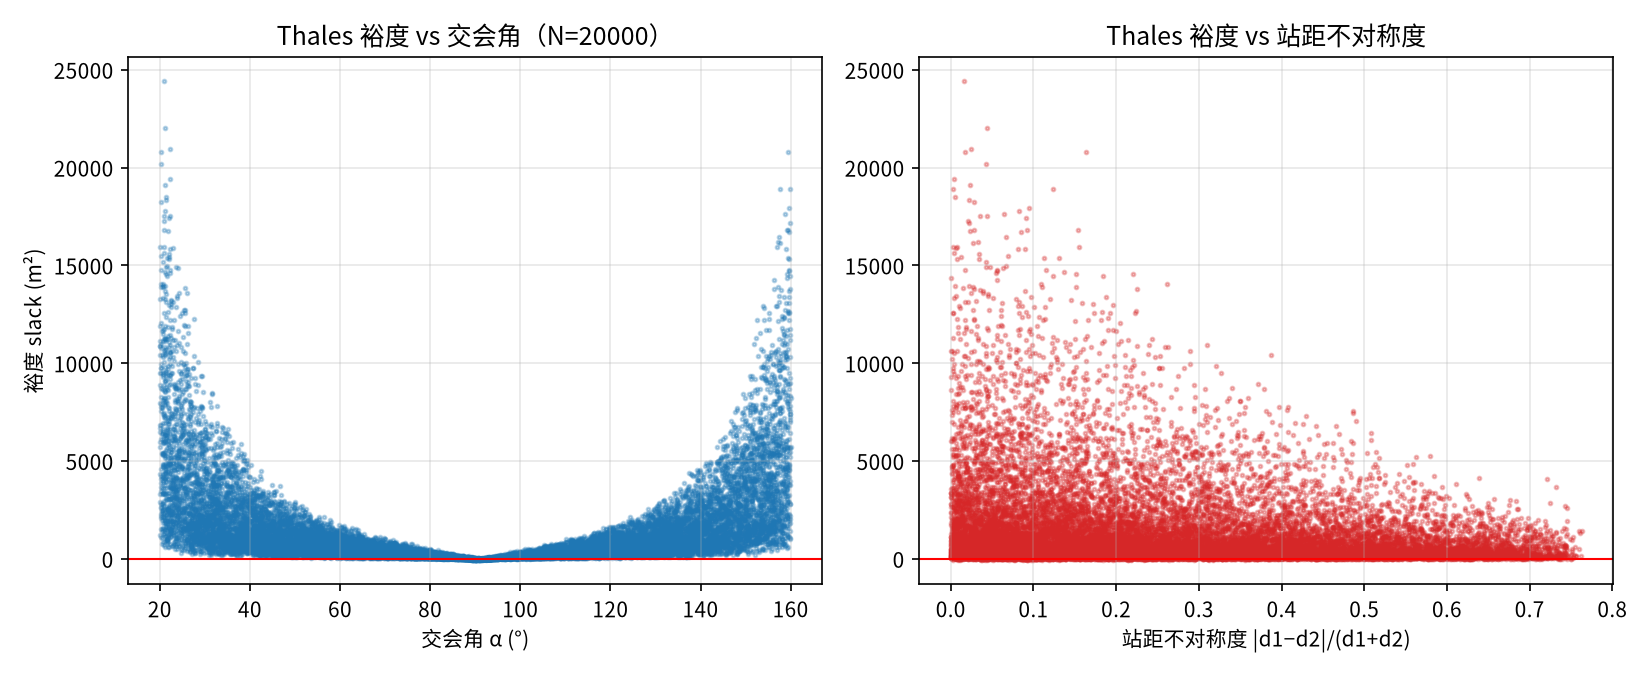
\includegraphics[width=\textwidth]{fig1.png}
  \caption{Thales 余量随交会角（左）与站距不对称度（右）的分布（$N=20000$）：不可覆盖样本集中在近正交构型。}
  \label{fig:thales}
\end{figure}

为说明临界性，构造精确鞍点：$\alpha=90\degr$、$d_1=d_2=1000\,$m、源位于中垂线上，此时可行集四顶点恰好内接于其直径圆，Thales 余量 $\slack=0$；在反对称误差的一个小邻域内，一侧方向仍覆盖、相反方向余量翻负（表 \ref{tab:saddle}）。这说明覆盖性在临界构型两侧改变，必须逐实例检验，任何关于一般情形都覆盖的断言都不成立。

\begin{table}[H]
  \centering
  \caption{临界鞍点构型（$\alpha=90\degr$，$d_1=d_2=1000\,$m）对反对称误差 $\pm\varepsilon$ 的响应}
  \label{tab:saddle}
  \begin{tabular}{ccccc}
    \toprule
    $\varepsilon$ (\degr) & $e_1=+\varepsilon,\ e_2=-\varepsilon$ & $\slack$ (m$^2$)
      & $e_1=-\varepsilon,\ e_2=+\varepsilon$ & $\slack$ (m$^2$) \\
    \midrule
    0.0  & 覆盖 & $-0.000$ & 覆盖   & $-0.000$  \\
    0.05 & 覆盖 & $2.131$  & 不覆盖 & $-41.767$ \\
    0.1  & 覆盖 & $4.269$  & 不覆盖 & $-39.499$ \\
    0.2  & 覆盖 & $8.568$  & 不覆盖 & $-34.986$ \\
    0.3  & 覆盖 & $12.899$ & 不覆盖 & $-30.506$ \\
    0.5  & 覆盖 & $21.654$ & 不覆盖 & $-21.641$ \\
    1.0  & 覆盖 & $44.125$ & 覆盖   & $0.000$   \\
    \bottomrule
  \end{tabular}
\end{table}

三个算例的结果（详见附录支撑材料 \verb|q1_results.md| 与图 \ref{fig:q1case}）：算例 1（常规交会）$d=70.3\,$m，覆盖；算例 2（三站）$d=62.2\,$m，覆盖；算例 3a（近平行视线）口径 \ding{172} 下 $W$ 无界，口径 \ding{173} 下 $d=1700\,$m、两个直径对均不满足式 (2)，不可覆盖；算例 3b（$1\degr$ 交会角病态薄片）$d=3001.7\,$m。

\begin{figure}[H]
  \centering
  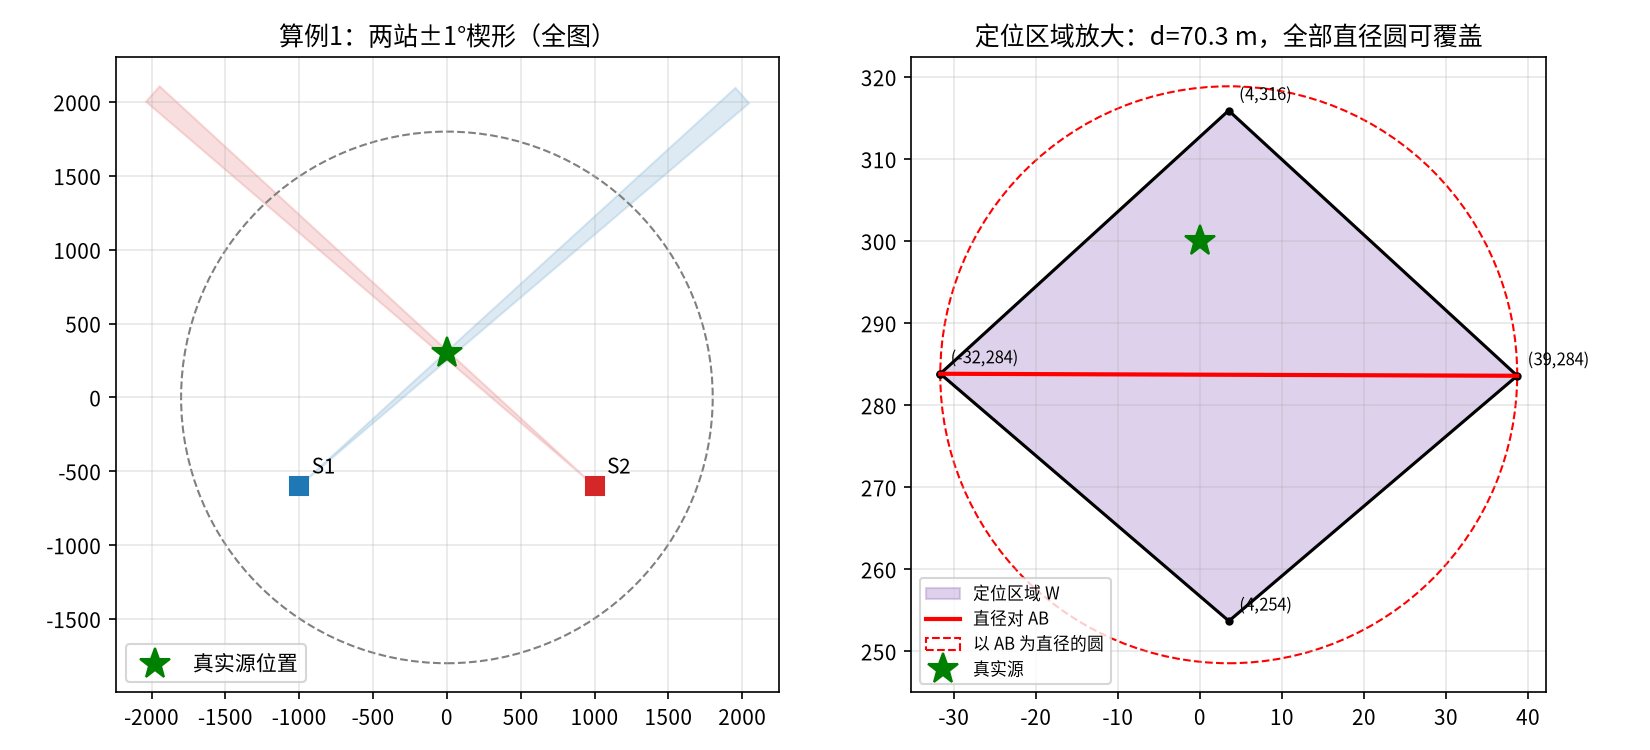
\includegraphics[width=\textwidth]{fig2.png}
  \caption{问题一算例 1：楔形交可行集与直径圆（覆盖成立）。}
  \label{fig:q1case}
\end{figure}

\textbf{问题一结论}：以定位区域直径为直径的圆\textbf{不一定}覆盖该区域。判别方法为：枚举全部直径对，逐一按式 (2) 检验 Thales 余量；全部通过则覆盖，否则存在该直径圆遗漏的顶点，不覆盖。该结论的适用范围是凸多边形可行集（两站情形即楔形交），抽样统计仅用于说明失败构型的分布特征。

\subsection{问题二：第二检测点的鲁棒选择}

\subsubsection{保证接收交集}

第一次观测后，可行集为
\begin{equation}
  F\ =\ W(S_1,\theta_1)\ \cap\ \disk(S_1,1500)\ \cap\ D_{1800},
\end{equation}
其中 $\disk(S_1,1500)$ 由接收半径上界给出。第二测点 $S_2$ 要对 $F$ 内任意可能源保证接收（距离不超过 $1000\,$m 下限），等价于
\begin{equation}
  S_2\in CR\ =\ \bigcap_{V\in\vertop(F)}\disk(V,1000).
\end{equation}
该等价性严格成立：对 $F$ 内任意点 $G=\sum\lambda_i V_i$（凸组合）与任意 $S_2\in CR$，由三角不等式 $\lVert G-S_2\rVert\le\sum\lambda_i\lVert V_i-S_2\rVert\le 1000$。反之若 $S_2\notin CR$，则存在顶点 $V$ 距 $S_2$ 超过 $1000\,$m，该顶点是合法源位置却不可保证接收。数值上各圆盘以 360 边形近似，得到的是保守内近似。

\subsubsection{鲁棒目标与求解算法}

第二测点的质量以第二次观测后的剩余区域度量。对源位置 $G\in F$ 与第二次误差 $e\in[-1\degr,1\degr]$，
\begin{equation}
  K_2(G,e)\ =\ F\ \cap\ W\bigl(S_2,\ \mathrm{br}(S_2\!\to\! G)+e\bigr)\ \cap\ \disk(S_2,1500),
\end{equation}
其中 $\mathrm{br}(S_2\!\to\! G)$ 为 $S_2$ 指向 $G$ 的方位角，$\disk(S_2,1500)$ 是第二测点自身可接收性的约束（实现中以 720 边形内接逼近，径向误差约 $0.014\,$m）。鲁棒目标为
\begin{equation}
  \Phi(S_2)\ =\ \max_{G\in F,\ e\in[-1\degr,1\degr]}\ \diam K_2(G,e).
\end{equation}
以直径而非 MEC 半径作为目标的原因：直径直接度量剩余可行域内任意两个可能真值之间的最大辨识误差，是定位不确定性的最坏尺度；MEC 半径只刻画以圆近似可行域时的清除可行性，作为清除判据在问题三、四中使用，二者分工不同。$\Phi$ 关于 $G$ 的凸性未证明，内层最大值只能离散采样：边界取顶点加每边 8 个内点、误差步长 $0.05\degr$。外层采用轻量\textbf{两层网格搜索}：粗网格（方位 $3\degr\times$ 半径 40 档）筛选，前 25 名候选局部细化（$0.5\degr\times 5\,$m），前 5 名再以全量加密样本（边界加密一档，另在 $F$ 内部按面积加权均匀采样 3 万点）逐一复核排序。因此报告值的意义是加密离散样本上的最坏值的最小者，不构成连续域的严格最优证明。计算量方面，粗网格 $120\times 40=4800$ 个候选中仅 25 个进入细化、5 个进入加密复核，内层采样支配耗时；粗筛只承担排序功能，最坏值一律以加密复核为准，避免了粗网格离散误差进入最终报告。

\subsubsection{算例结果}

算例设定 $S_1=(-800,-1000)$，$\theta_1=53.5\degr$，真源 $(0,100)$。结果：

\begin{itemize}[leftmargin=2em,itemsep=3pt]
  \item 最优候选 $S_2^{*}=(-727.8,-2.9)$（方位 $133.5\degr$，$\rho^{*}=543.3\,$m），加密复核最坏直径 $\Phi_{\mathrm{dense}}=\textbf{111.7\,m}$，为一次测量区域尺度（$1500\,$m）的 \textbf{7.4\%}；
  \item 收敛性复核：边界样本加密一档后差 $0.00\,$m；考虑 $\Phi$ 凸性未知，另在 $F$ 内部按面积加权均匀采样 3 万点（误差步长 $0.05\degr$），内部最坏值 $111.7\,$m 未超过边界值，结论在边界与内部联合采样下稳定；
  \item $S_2^{*}$ 与第一示向度的垂直方向（$144\degr/324\degr$）偏差 $10.0\degr$：与适度距离上垂直交会的定性认识一致，但受 $CR$ 截断与网格离散影响，不构成垂直最优的证明；
  \item 对照：$S_2$ 位于第一示向度线上时交会几何退化，修正口径下定位区域被 $F$ 截断为细条，$\Phi=750.1\,$m（有限但定位效果很差）；无保证接收约束的 $\rho=1500\,$m 垂直点 $\Phi\approx 54\,$m，仅作对照，说明保证接收约束付出了代价。
\end{itemize}

\begin{table}[H]
  \centering
  \caption{加密复核下前 5 个候选第二测点的鲁棒目标值（最优解附近目标面平坦）}
  \label{tab:q2top5}
  \begin{tabular}{cccc}
    \toprule
    $S_2$ (m) & 方位 (\degr) & $\rho$ (m) & $\Phi_{\mathrm{dense}}$ (m) \\
    \midrule
    $(-727.8,\,-2.9)$ & 133.5 & 543.3 & \textbf{111.717} \\
    $(-734.7,\,-2.6)$ & 134.0 & 548.3 & 111.721 \\
    $(134.8,\,-646.0)$ & 333.0 & 548.3 & 111.721 \\
    $(-721.0,\,-3.3)$ & 133.0 & 538.3 & 111.733 \\
    $(-741.7,\,-2.4)$ & 134.5 & 553.3 & 111.745 \\
    \bottomrule
  \end{tabular}
\end{table}

\begin{figure}[H]
  \centering
  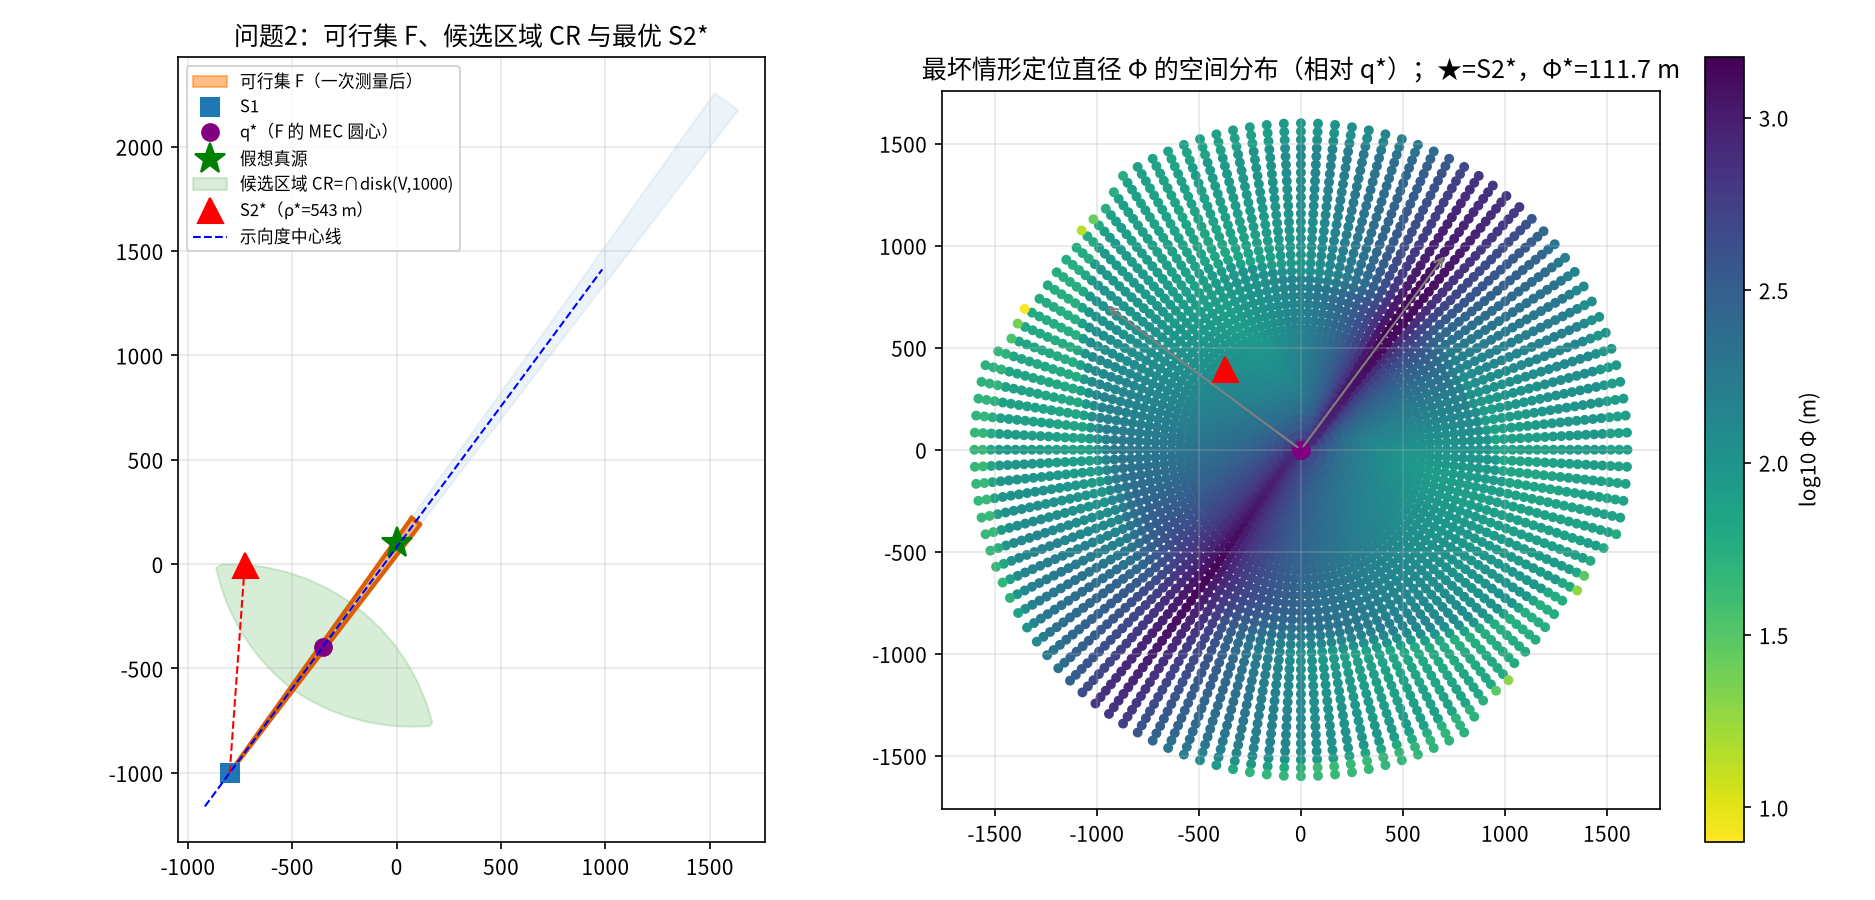
\includegraphics[width=\textwidth]{fig3.png}
  \caption{问题二：可行集 $F$、保证接收交集 $CR$ 与最优第二测点 $S_2^{*}$。}
  \label{fig:q2}
\end{figure}

\textbf{问题二结论}：算例的最优第二测点为 $S_2^{*}=(-727.8,-2.9)$，对应剩余区域最坏直径 \textbf{111.7\,m}（一次测量尺度的 \textbf{7.4\%}）。该值是加密离散样本意义下的最坏值最优，其收敛性经边界与内部联合采样复核；垂直交会仅作为定性先验进入候选生成，不作为最优性依据。

\subsection{问题三：全向源的搜索、定位与清除}

\subsubsection{覆盖层：九点布局与发现保证}

全向源的可接收区域是圆盘，故测点集只需对目标圆域形成半径不超过 $1000\,$m 的覆盖。采用中心加半径 $1000\,$m 正八边形共 9 个测点：中心覆盖半径 $1000\,$m 的内圆；圆域边界上最坏点位于相邻环点角平分方向，其到最近环点的距离
\begin{equation}
  \sqrt{1800^{2}+1000^{2}-2\cdot 1800\cdot 1000\cdot\cos 22.5\degr}\ \approx\ 956\ \mathrm{m}\ <\ 1000\ \mathrm{m},
\end{equation}
故任意全向源（接收半径 $\ge 1000\,$m）至少被一个测点检出，发现保证成立（图 \ref{fig:q3layout}）。需要说明的是，该保证只是单站的：边界上与环点同方位的源（如 $1800\vect{u}(0\degr)$）距相邻环点约 $1302\,$m，超出接收半径下界，此时仅单站检出，可行集为 $2\degr$ 楔形，定位由补测管线继续收敛完成，不依赖双站交会。

式 (8) 的最坏点结论可以严格化而不仅是逐点验证。设边界点 $P(t)=1800\vect{u}(t)$，$t\in[0\degr,45\degr]$ 落在两相邻环点（方位 $0\degr$ 与 $45\degr$，半径 $1000\,$m）之间的扇区。$P(t)$ 到其中一个环点的距离
\[
  f(t)=\sqrt{1800^{2}+1000^{2}-2\cdot 1800\cdot 1000\cos t}
\]
的被开方数对 $t$ 的导数为 $2\cdot 1800\cdot 1000\sin t\ge 0$，故 $f$ 在 $[0\degr,45\degr]$ 上单调递增；点 $P(t)$ 到最近环点的距离为 $\min\{f(t),\,f(45\degr-t)\}$，由对称性与单调性，其最大值在 $f(t)=f(45\degr-t)$ 即 $t=22.5\degr$ 处取得，代入得 $956\,$m。覆盖余量 $1000-956=43.6\,$m，且该余量对扇区内所有边界点成立，使最坏点位于角平分方向这一结论从直觉升级为单调性论证。

\begin{figure}[H]
  \centering
  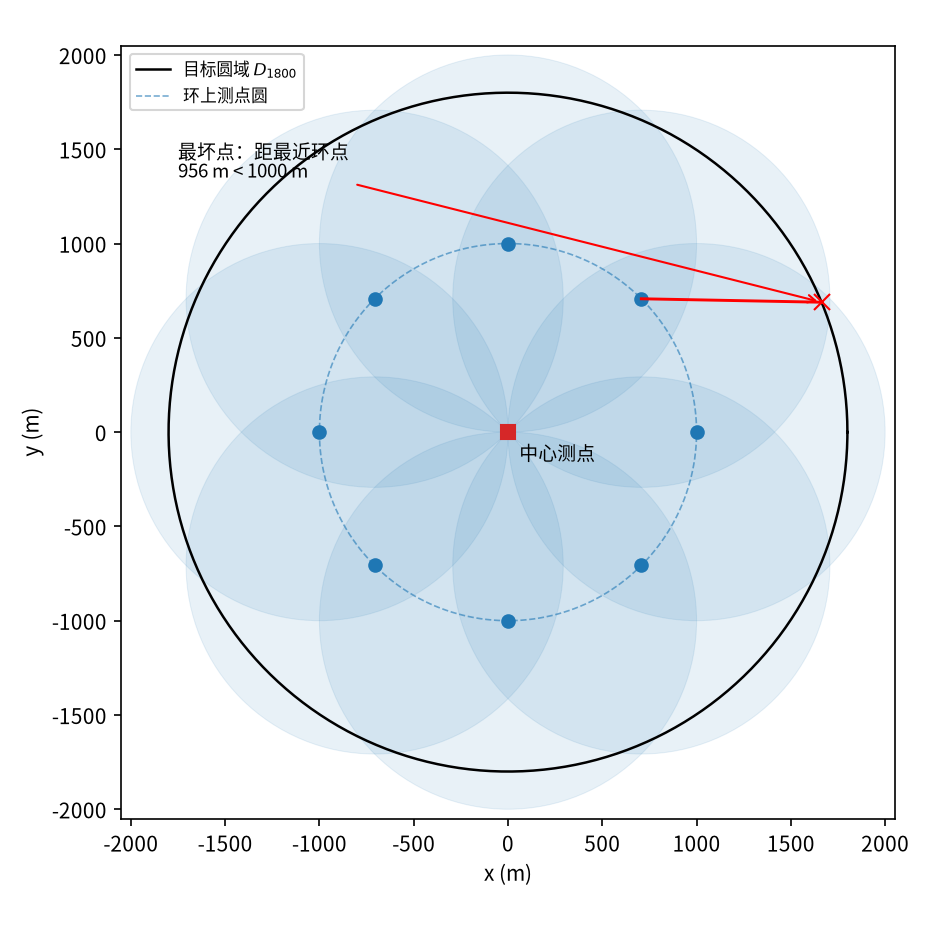
\includegraphics[width=0.72\textwidth]{fig4.png}
  \caption{问题三九点布局：8 个 $1000\,$m 接收盘对目标圆域的覆盖与边界最坏点几何。}
  \label{fig:q3layout}
\end{figure}

\subsubsection{定位与清除层}

每个测点按蛇形顺序扫描全部信道。对检出信号信道 $c$，用半平面交维护可行集并计算最小覆盖圆（MEC）。收敛闸门取
\begin{equation}
  r_{\mathrm{MEC}}\ \le\ 19.75\ \mathrm{m}\ =\ \texttt{CLEAR\_RADIUS}-0.25\ \mathrm{m}:
\end{equation}
$20\,$m 为清除半径，$0.25\,$m 裕度覆盖可行域多边形近似与浮点误差。$r_{\mathrm{MEC}}\le 19.75\,$m 时圆心到真实源距离上界即 $19.75\,$m，清除必然成功，这是清除环节唯一的确定性判据。

补测点取当前 MEC 圆心：清除点本就是收敛后的圆心，在圆心测向等于顺路，且一次方向读数给出半宽约 $r_{\mathrm{MEC}}\tan 1\degr$ 的窄带，收敛速度优于在 $450\,$m 视线垂直点补测。该设计经配对消融实验验证（同批 200 局）：平均每源耗时 $402.0\to 359.4\,$s，下降 10.6\%；不宣称圆心补测理论最优。连续 \verb|no_signal| 时启用折半逼近回退分支。收敛且机器狗距圆心不超过 $400\,$m 时就地清除（收敛即清，闸值敏感性见 6.3 节）；全部收敛源按最近邻初解加 2-opt 局部改进排序清除（Croes, 1958）；2-opt 只保证局部最优，实测路径长度已非瓶颈。

\subsubsection{调度层与异常降级}

三项调度措施：\textbf{全局交错补测}，即补测阶段每步从所有未收敛信道选距当前位置最近的候选点，消除按信道序号折返；\textbf{跳测判定}，即已检出信道的可行集若完全在当前测点 $1500\,$m 之外（接收半径上界），该次测量必然 \verb|no_signal|，直接跳过；已清除信道亦跳测。该判定可证明安全（内点距离偏小只会少跳、不会误跳），配对 100 局平均每局省 $176.5\,$s（$-3.3\%$）。\textbf{异常降级}，即所有动作校验 \verb|accepted| 标志；动作被拒或网络重试耗尽时按阶段降级：搜索中断保留已有示向度继续，单信道补测失败只放弃该信道，清除失败与时间不足的残留信道全部计入 \verb|failed_channels| 上报，保证 discovered $=$ cleared $\cup$ failed 的分类完备性，不弃局。故障注入回归 100 项（对 \verb|measure|/\verb|clear|/\verb|exit| 注入拒绝与网络耗尽两类故障）全部通过。

\subsubsection{结果}

离线回归（md5 确定性可复现）：配对 200 局加全新 300 局共 500/500 全清，平均每源 $359.4\,$s；相同随机案例下，采用 MEC 圆心补测与全局交错调度的策略较垂直侧移补测对照策略的 $402.0\,$s/源降低 10.6\%。官方模拟器真机演练 12 局 163/163 全清，其中采用本文最终策略的 6 局每源 $295.1\sim 348.5\,$s；正式测试 3 局 40/40 全清，平均 $367.1\,$s/源（逐局数据见表 \ref{tab:formal}）。虚拟时间结构经演练日志反推核实：每次测量恰 $6\,$s、移动 $5\,$m/s、清除约 $6\,$s；六局正式测试的完整时间构成分解见图 \ref{fig:timebreak}：移动占 $71\%\sim 81\%$、测量占 $17\%\sim 28\%$、清除不足 2\%，与移动主导、布局优先的建模判断一致。图 \ref{fig:q3traj} 还原了正式测试第三局（16 源）的完整动作轨迹：机器狗先沿九点布局完成扫描，随后按全局交错补测逐源收敛、清除，153 次测量与 16 次清除的位置序列与本节策略描述一一对应。

\begin{figure}[H]
  \centering
  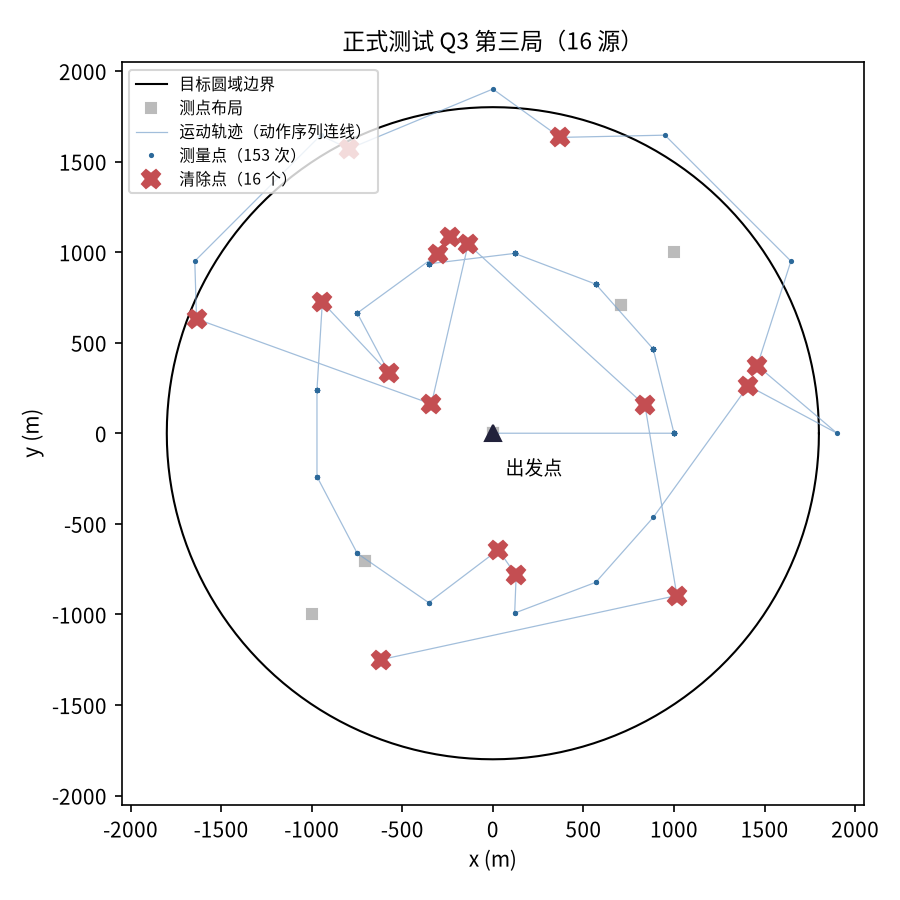
\includegraphics[width=0.72\textwidth]{fig5.png}
  \caption{正式测试 Q3 第三局（16 源）真实动作轨迹（由日志 169 个动作坐标还原）：测量点、清除点与运动路径。}
  \label{fig:q3traj}
\end{figure}

\subsection{问题四：混合源的搜索、定位与清除}

\subsubsection{保证层级结构}

定向源的加入使发现成为非平凡问题，我们把问题四的保证组织为四层，并严格区分确定性保证与实验验证两类命题：

\begin{itemize}[leftmargin=2em,itemsep=3pt]
  \item \textbf{\ding{172}发现层（确定性保证）}：26 点环形骨架对任意源位置、任意发射朝向保证检出；
  \item \textbf{\ding{173}常规清除层（确定性判据）}：MEC 半径 $\le 19.75\,$m 时出手必中；
  \item \textbf{\ding{174}极端兜底层（几何确定性）}：$17.2\,$m 三角细网格，在补测用尽且 MEC 仍未收敛的病态分支下，候选网格中必存在可接收且可成功清除的测点；在线程序在剩余时间允许时执行该扫描；
  \item \textbf{\ding{175}效率调度层（不承担保证责任）}：交错补测、顺路清除、跳测等效率措施。
\end{itemize}

发现后能全部定位并清除在 \ding{172}\ding{173} 正常工作的前提下不属于定理范围，由大规模仿真与官方模拟器实测验证；论文与答辩表述为：确定性保证发现，病态情形有兜底保证，定位清除经仿真与实测验证，不使用确保清除所有源一类表述。四层在执行上的关系是：第 \ding{174} 层只在补测用尽且 MEC 未收敛的分支上触发，正常情形零触发。

\subsubsection{发现层：26 点环形骨架与弧判据}

定向源可检出当且仅当存在测点 $S$ 使 $|S-G|\le R$ 且 $(S-G)\cdot\vect{u}(\varphi)\ge 0$。对固定源位置 $G$，记其 $1000\,$m 内可用测点的方位集合为 $\Theta(G)$，则对任意朝向 $\varphi$ 均可检出的条件等价于
\begin{equation}
  \maxGap\bigl(\Theta(G)\bigr)\ \le\ 180\degr,
\end{equation}
其中等号对应测点恰落在半圆边界的情形；本文数值结果均有约 $3.2\degr$ 的严格正裕度，故开、闭边界约定不改变布局结论。

\textbf{式 (10) 的等价性证明}：固定 $G$，记可用测点（$|S-G|\le R$）的方位集合为 $\Theta(G)$。题目的接收半圆包含边界，因此某一朝向不可检出，当且仅当全部可用测点严格落在其接收半平面之外；在圆周方位上，这等价于存在一段大于 $180\degr$ 的空弧。取逆否并对朝向量化，任意朝向均可检出当且仅当最大方位空隙不超过 $180\degr$。本文扫描得到的最坏值为 $176.21\degr$，远离等号边界。

搜索骨架取\textbf{原点 $+$ 13 点 @$1000\,$m}（$27.7\degr$ 间距）$+$ \textbf{12 点 @$1900\,$m}（$30\degr$ 间距）共 26 点：内环覆盖朝内与切向定向源，外环覆盖贴边朝外源，贴边最坏构型（源在 $1800\,$m 边界、朝向径向向外、位于两外环点正中）的半平面裕度为 $1900\cos 15\degr-1800=35.2\,$m $>0$（图 \ref{fig:q4layout}）。$1900\,$m 环测点在目标圆域外，其合规依据是：题目正文以 $1800\,$m 圆限制干扰源分布区域，附件 1 明确机器狗位置不构成约束；且数学上该外环不可省略：$D_{1800}$ 边界点无法被任何完全场内点集的凸包包含。

\textbf{无盲区验证（三重独立 $+$ 分层闭合）}：式 (10) 是含 $\max$ 的非凸判据，封闭形式的分情形证明繁琐且易漏，因此先用三种独立离散方式交叉复核，再用分层 Lipschitz 界处理格点之间与判据跳变边界：(i) 精确穷举（朝向解析精确，网格 $0.5\,$m $\times$ $0.25\degr$）：盲区 0 格，最小角裕度 $3.198\degr$，最坏最近距 $585.2\,$m；(ii) 独立实现复核（直角网格 $5\,$m，407\,455 个源位置）：盲区 0，最坏空隙 $176.21\degr<180\degr$；(iii) 边界薄缝检查：离散验证的共同理论缺口在判据的不连续点，即测点恰好出界的 $|S-G|=1000\,$m 边界。对全部 26 个边界圆外侧 $0.02\sim 2\,$m、每圆 36\,000 个方位点直查，最坏角裕度 $3.218\degr$。三套验证互证：薄缝不存在，零盲区结论在判据不连续点上同样成立（图 \ref{fig:q4scan}）。三套验证的口径差异见表 \ref{tab:triple}：采样方式与朝向处理互不相同，最坏值却落在同一量级，这正是独立验证的含义。

\begin{table}[H]
  \centering
  \caption{发现层无盲区的三重独立验证口径对照（最坏结果两两独立取得）}
  \label{tab:triple}
  \begin{tabular}{@{}p{3.2cm}p{4.6cm}p{5.2cm}@{}}
    \toprule
    验证通道 & 源位置采样 / 朝向处理 & 最坏结果 \\
    \midrule
    (i) 精确穷举 & $0.5\,$m 网格 $\times$ $0.25\degr$ 方位；朝向解析精确
      & 盲区 0 格；最小角裕度 $3.198\degr$；最坏最近距 $585.2\,$m \\[4pt]
    (ii) 独立实现复核 & 直角 $5\,$m 网格（407\,455 点）；弧判据（式 (10)）
      & 最坏空隙 $176.21\degr<180\degr$ \\[4pt]
    (iii) 边界薄缝直查 & 26 个边界圆外侧 $0.02\sim 2\,$m；每圆 36\,000 方位点
      & 最坏角裕度 $3.218\degr$ \\
    \bottomrule
  \end{tabular}
\end{table}

\textbf{从离散扫描到连续域结论（分层 Lipschitz 闭合）}：在可用测点集不变的开区域内，$\Theta(G)$ 中每个方位随 $G$ 移动的漂移速率不超过 $1/d$（$d$ 为该测站到 $G$ 的距离），于是对采样格点 $G_0$ 与半格距 $h$ 邻域内的任意 $G$，
\begin{equation}
  \bigl|\maxGap(G)-\maxGap(G_0)\bigr|\ \le\ \delta\Bigl(\frac{1}{d_i}+\frac{1}{d_j}\Bigr)\ \le\ \frac{2h}{d_{\mathrm{end}}(G_0)},
\end{equation}
其中 $d_{\mathrm{end}}(G_0)$ 为最大空隙两端测站到 $G_0$ 距离的较小者。按可用集变化和端点退化把 $D_{1800}$ 分四层：\textbf{(1) 主体区}用 $0.5\,$m 网格检查 4027 万点，最小闭包量 $+3.32\degr$；\textbf{(2) 26 个检出圆的 $\pm 0.4\,$m 条带}用 $0.02\,$m$\times 0.02\degr$ 网格检查 1123 万点，跳变两侧分别闭合，最小闭包量 $+3.12\degr$；\textbf{(3) 14 个场内测站的 $30\,$m 邻域}检查 6048 万点。近站端点由邻接弧解析界处理：外环可用站相对朝外空段中轴的偏离不超过约 $19\degr$，故相邻空隙不超过 $120\degr$、裕度至少 $60\degr$；其余端点距源不小于 $450\,$m，采样最小裕度 $51.4\degr$，层内漂移不超过 $0.012\degr$；\textbf{(4) 全部 361 个圆--圆或圆--域界交点的 $\pm 0.65\,$m 邻域}用 $0.005\,$m 网格检查 2289 万点，最小闭包量 $+3.19\degr$。四层覆盖目标圆域且闭包量均为正，故 $\maxGap(G)<180\degr$ 在连续域处处成立，保守最小角裕度下界约为 \textbf{3.1\degr}。全部点数、极值位置和闭包量由同一程序写入 \verb|q4_closure_pointwise.json|，最终标志为 \verb|all_closed=true|。

\begin{figure}[H]
  \centering
  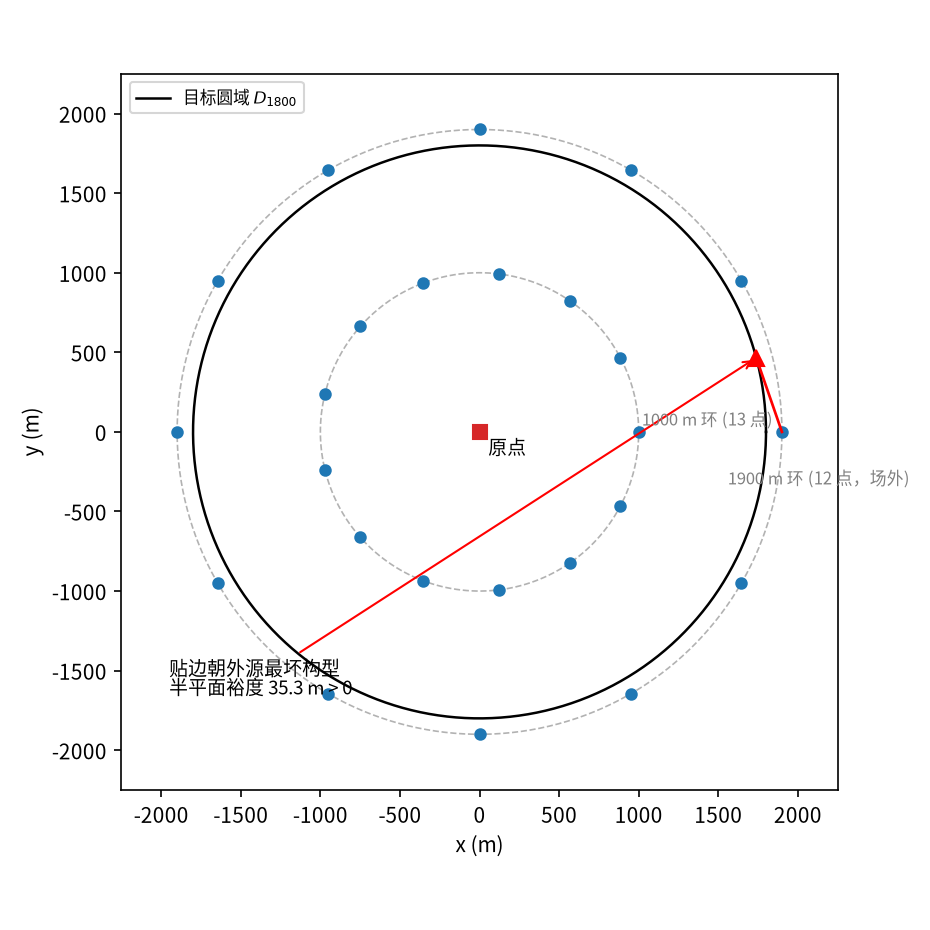
\includegraphics[width=0.72\textwidth]{fig6.png}
  \caption{问题四 26 点环形骨架与贴边朝外源最坏构型（半平面裕度 $35.2\,$m）。}
  \label{fig:q4layout}
\end{figure}

\begin{figure}[H]
  \centering
  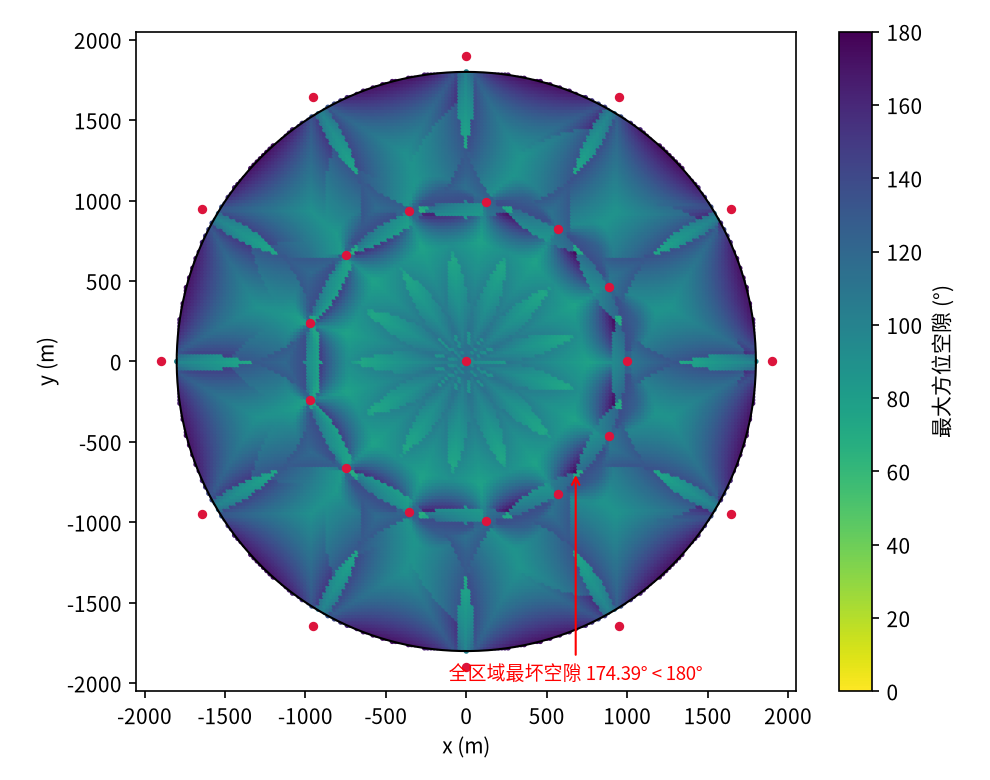
\includegraphics[width=0.8\textwidth]{fig7.png}
  \caption{弧判据多分辨率扫描：$20\,$m 网格最坏值为 $174.4\degr$，$5\,$m 网格为 $176.2\degr$，检出圆条带加密扫描为 $176.8\degr$；各离散验证均未发现盲区。}
  \label{fig:q4scan}
\end{figure}

\subsubsection{常规清除与效率调度}

发现后的定位、清除与调度沿用问题三框架：楔形交可行集、MEC 收敛闸 $19.75\,$m、MEC 圆心补测、深度阶梯与垂直交会候选、折半逼近回退、全局交错补测、收敛即清、顺路清除（绕路上限 $400\,$m）与跳测判定。\verb|no_signal| 的三义性（空信道、超半径、覆盖外）使其不能用于新增楔形，仅作不可用于定位的观测记录。

\subsubsection{极端兜底层：$17.2\,$m 三角细网格}

某信道 16 次补测用尽且 $r_{\mathrm{MEC}}>19.75\,$m 时，进入细网格兜底：对该信道正测向可行集外扩 $20\,$m 的区域铺设间距 $17.2\,$m 的三角格，按蛇形序逐点测量、遇信号就地清除。其保证由夹逼不等式给出：对任意源位置 $G$ 与任意朝向 $\vect{u}(\varphi)$，理想点 $y=G+10\vect{u}(\varphi)$ 距 $G$ 恒为 $10\,$m，三角格覆盖半径 $\rho=17.2/\sqrt{3}\approx 9.93\,$m，故存在格点 $s$ 使 $|s-y|\le\rho$，从而
\begin{align}
  |s-G|&\ \le\ 10+9.93\ =\ 19.93\ \mathrm{m}\ <\ 20\ \mathrm{m}\quad\text{（清除必成功）},\\
  (s-G)\cdot\vect{u}(\varphi)&\ \ge\ 10-\rho\ =\ 0.07\ \mathrm{m}\ >\ 0\quad\text{（$s$ 在前向半平面内，测量必有信号）}.
\end{align}
两个不等式对 $G$ 与朝向均无假设，故兜底层提供的是\textbf{几何完备性}：候选网格中必存在一个既能收到信号、又处于清除半径内的测点；若该网格被完整扫描，则必能到达该点。程序执行层面，该层受时间保护（预留 $180\,$s，不足则中止并在 summary 如实上报），即在线程序在剩余真实时间允许时执行该兜底策略；\textbf{正常情形零触发}：800 局离线回归与 10 局真机实验均未触发；强制触发单元测试（把补测上限压至 1 次）中触发即清除，验证了不等式在本模拟器语义下的有效性：补测用尽的信道均能正确转入细网格兜底流程，并在检测到满足条件的网格点后完成清除，该分支责任闭环完整。

\subsubsection{布局选型：搜索布局比较}

为选择发现层布局，比较三种候选：36 点 $6\times 6$@$720\,$m 方格、27 点等边三角格网与 26 点环形骨架。27 点三角格在混合 200 局中较 36 点方格慢 7.5\%（855.0 对 $795.1\,$s/源），测点数更少的三角格网反而更慢，说明发现层不能孤立地以测点数评价。在同一套二三四层、仅更换发现层的条件下，对 36 点方格与 26 点环形骨架各跑离线配对 400 局：26 点环形平均每源 $595.4\,$s，较 36 点方格的 $729.1\,$s 快 \textbf{18.3\%}；全定向压力 100 局快 14.9\%、全向压力 100 局快 24.3\%。真机同源数配对方向一致：11 源局 $841.0\to 644.1\,$s/源（$-23.4\%$），13 源局 $695.7\to 598.5\,$s/源（$-14.0\%$），两种布局全清率无差异、兜底均零触发。

\textbf{机制解释}：\textbf{稀疏骨架的价值取决于补测管线强度}。26 点环形把负担从扫描期（巡视路程 25\,709\,m 降至 18\,678\,m、扫描测量 720 次降至 520 次，均为确定性节省）转移到补测期（每源示向度更少）；补测管线较弱时该代价无法吸收（27 点三角格情形），管线足够强（交错补测、收敛即清、跳测齐备）时红利即可兑现。36 点与 27 点三角格的对照混合了布局差异与管线差异，不能外推到 26 点环形。故问题四采用 26 点环形布局（图 \ref{fig:layoutcmp}）。

\begin{figure}[H]
  \centering
  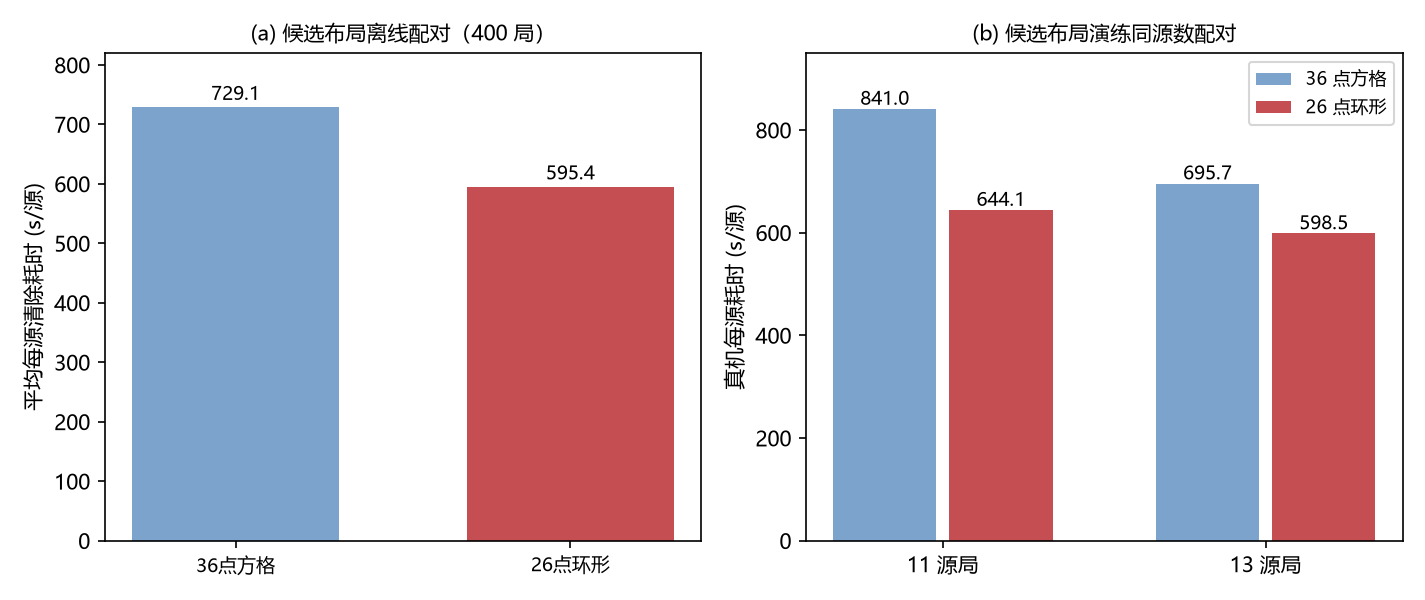
\includegraphics[width=\textwidth]{fig8.png}
  \caption{36 点方格与 26 点环形两种候选布局的对照：(a) 400 局离线配对回归；(b) 模拟器演练中的同源数配对。}
  \label{fig:layoutcmp}
\end{figure}

\subsubsection{结果}

离线回归：26 点环形布局混合 400 局 400/400 全清、平均 $595.4\,$s/源；全定向 100 局 $668.6\,$s/源、全向 100 局 $513.5\,$s/源（均全清）。在相同定位、清除与调度机制下，26 点环形较 36 点方格的 $729.1\,$s/源降低 18.3\%，对照见图 \ref{fig:layoutcmp}。模拟器演练 15 局 200/200 全清，其中采用 26 点环形布局的 3 局每源 $527.1\sim 644.1\,$s；正式测试 3 局 37/37 全清，平均 $550.2\,$s/源（逐局数据见表 \ref{tab:formal}）。全部正式测试均正常退出，零拒绝动作、零失败信道，兜底层保持休眠。图 \ref{fig:q4traj} 还原正式测试第二局（13 源）的动作轨迹：内环 $1000\,$m 测点承担绝大部分检出，外环 $1900\,$m 测点仅用于覆盖贴边朝外源，291 次测量与 13 次清除的位置序列与本节策略描述一致。

\begin{figure}[H]
  \centering
  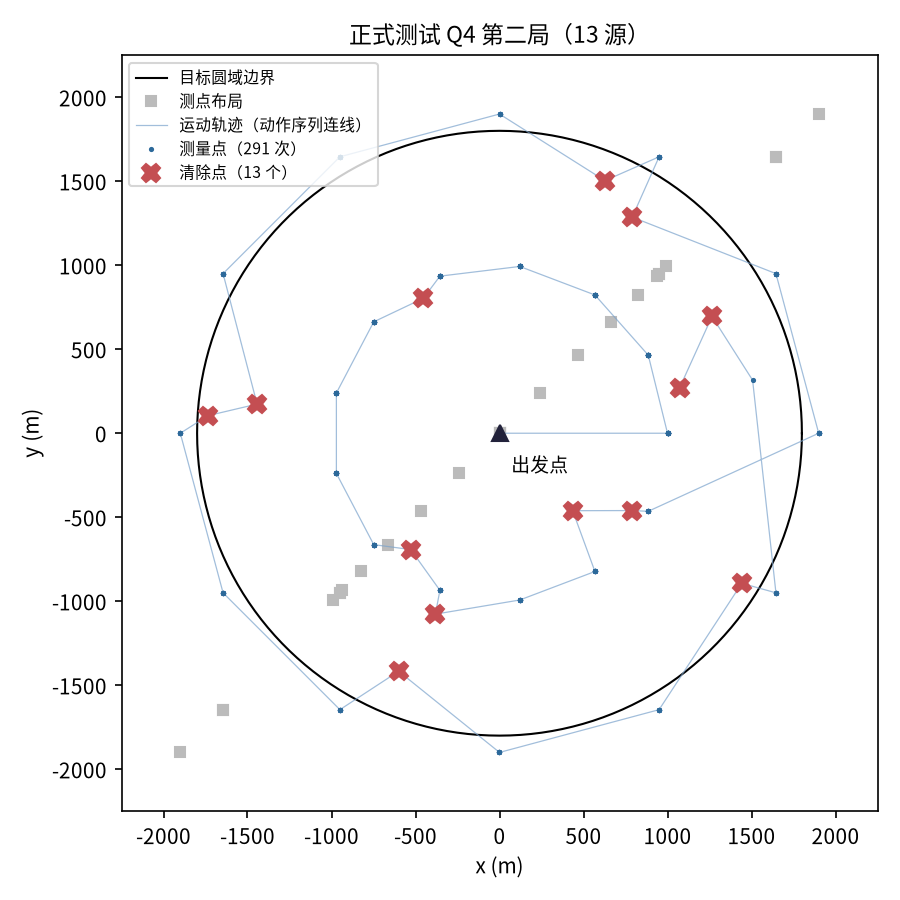
\includegraphics[width=0.72\textwidth]{fig9.png}
  \caption{正式测试 Q4 第二局（13 源）真实动作轨迹（由日志 304 个动作坐标还原）：灰色方块为含 $1900\,$m 场外环的完整骨架。}
  \label{fig:q4traj}
\end{figure}

%========================== 六、模型的检验与敏感性分析 ==========================
\section{模型的检验与敏感性分析}

\subsection{虚拟时间模型的核实}

由演练日志反推的时间模型（测量 $6\,$s、移动 $5\,$m/s、清除约 $6\,$s）在 33 局真机实验中保持一致：真机每源耗时与离线回归值吻合（问题三正式 367.1 对离线 $359.4\,$s/源；问题四正式 550.2 对离线 $595.4\,$s/源）。这说明离线模拟器复现了官方模拟器的主要运行特征（关键动作计时一致、每源耗时处于相近区间），因而离线调参结论可以迁移；本文不主张两个模拟器在所有输入与异常路径上语义等价。对六局正式测试的动作日志逐动作分解虚拟时间（图 \ref{fig:timebreak}）：六局移动占比均不低于 71\%（最高 81\%），清除合计不足 2\%，时间预算几乎全部消耗在巡视移动上，这是覆盖层测点少而精与调度层压缩路程两项设计的共同经验依据。

\begin{figure}[H]
  \centering
  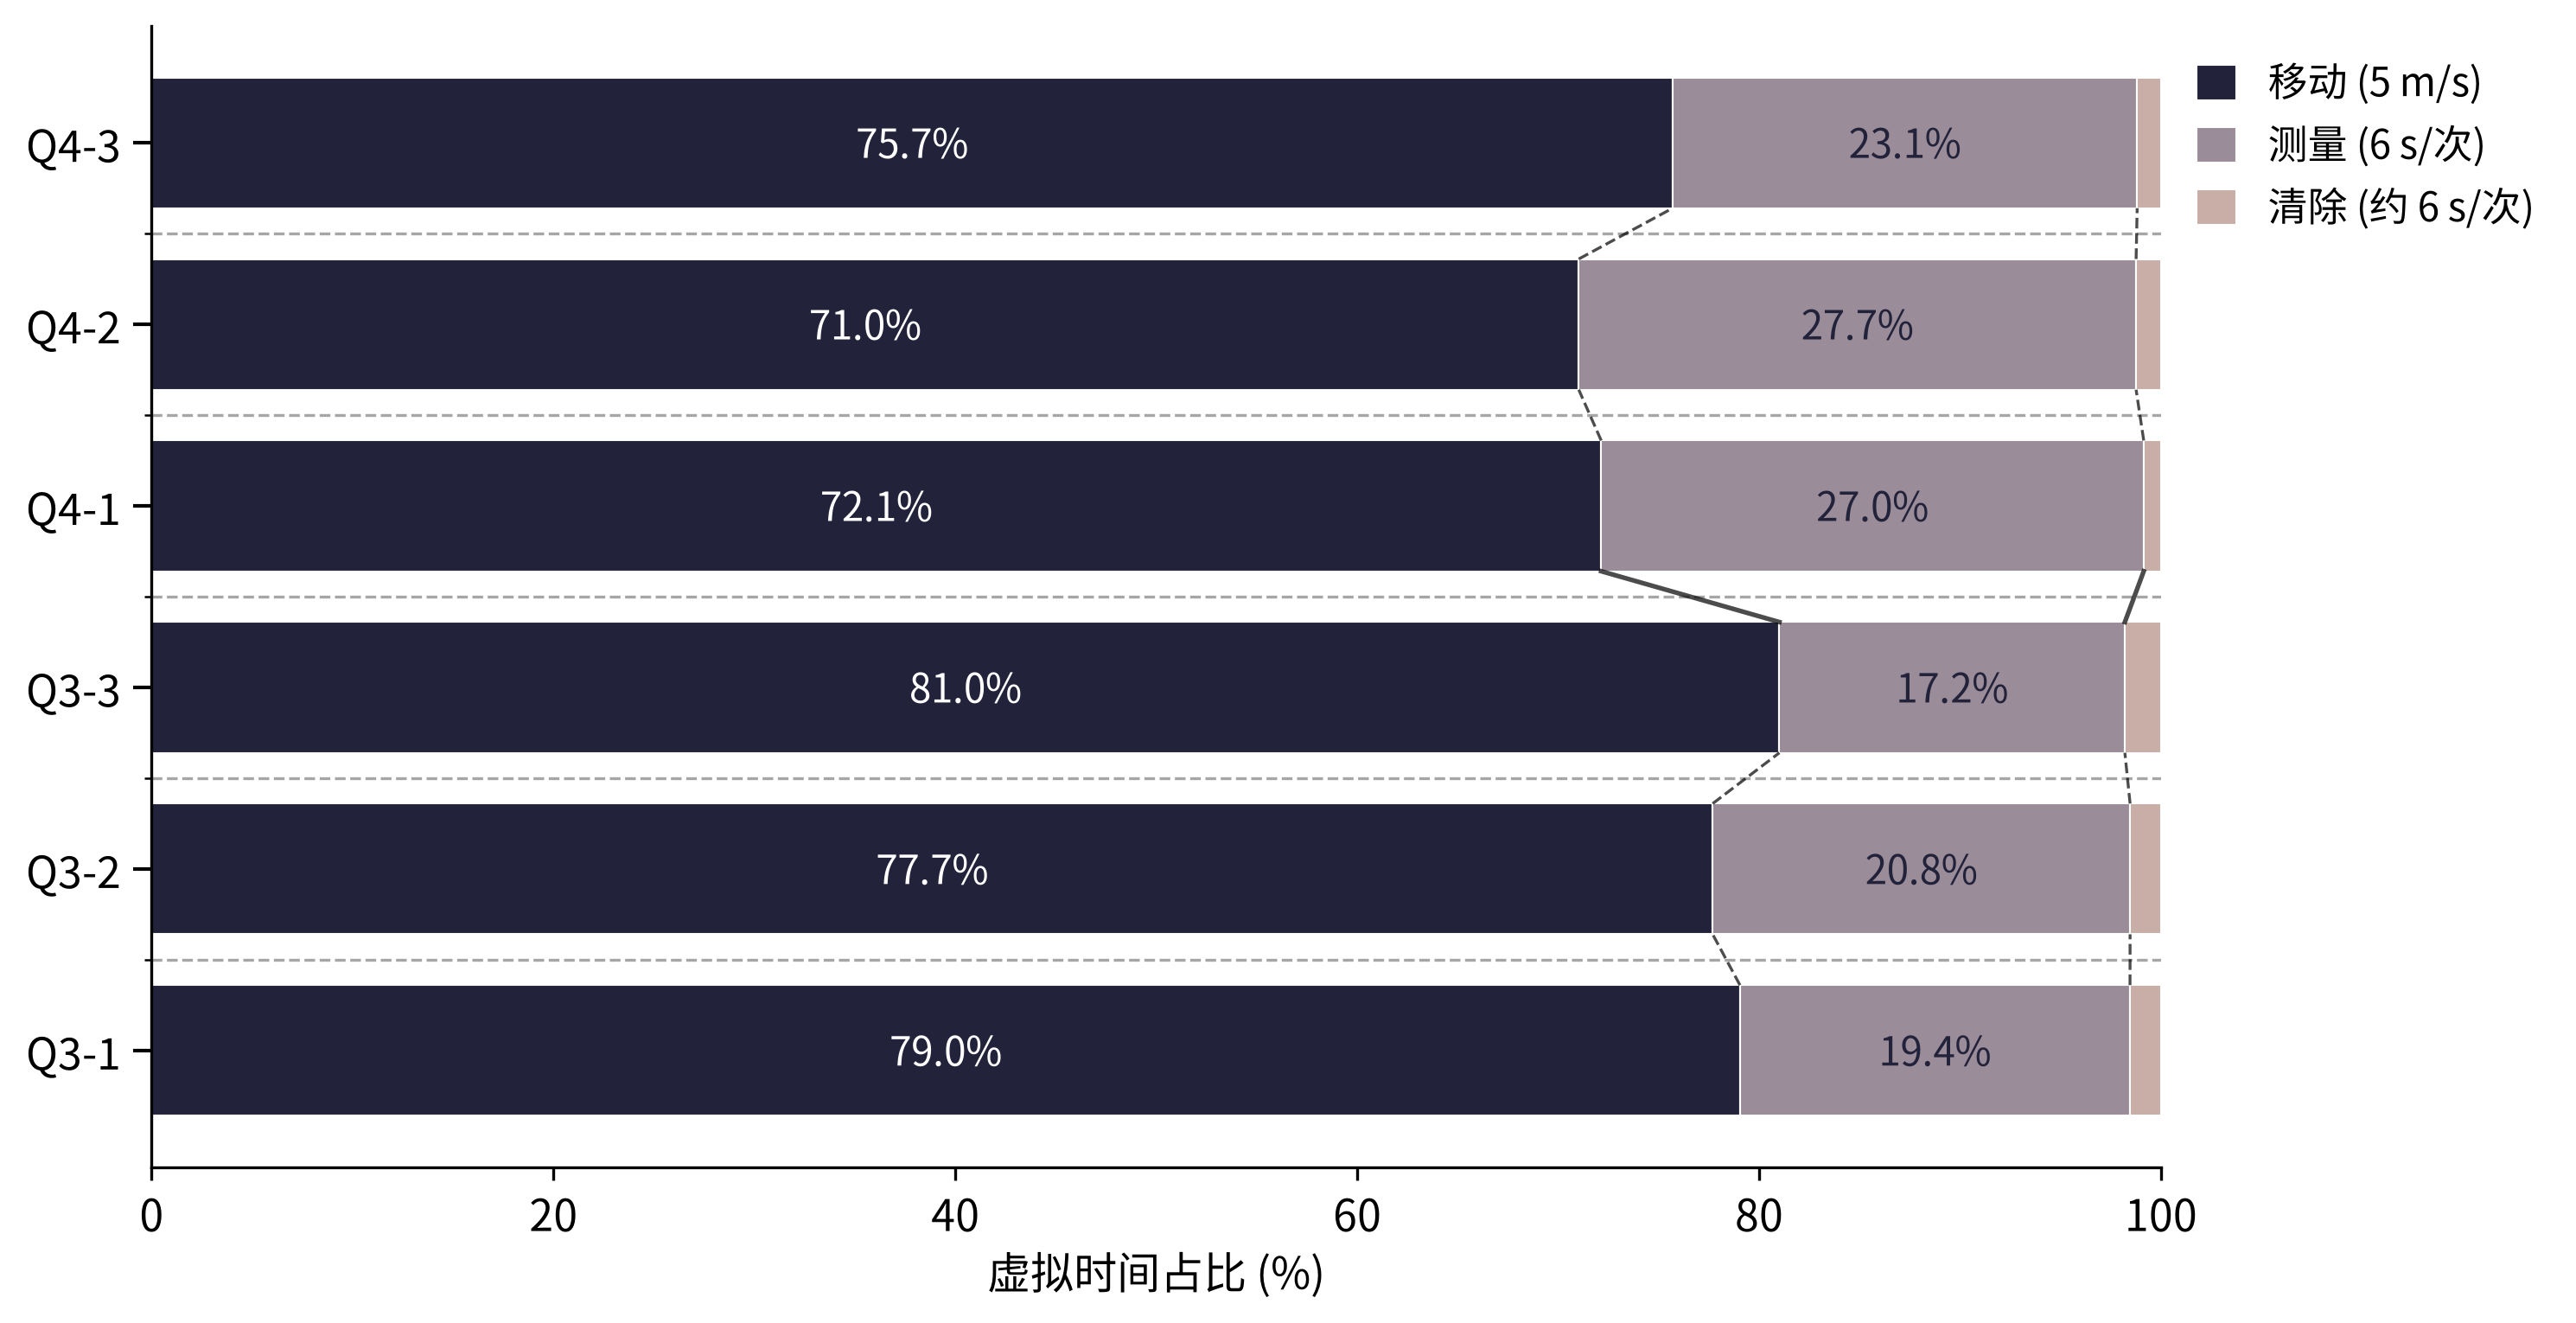
\includegraphics[width=\textwidth]{fig10.png}
  \caption{六局正式测试的虚拟时间构成（由动作日志逐项分解）：移动占 $71\%\sim 81\%$，测量占 $17\%\sim 28\%$，清除不足 2\%。}
  \label{fig:timebreak}
\end{figure}

\subsection{真机演练的逐局证据}

除正式测试外，我们在官方模拟器上累计完成 27 局真机演练（问题三 12 局、问题四 15 局）。图 \ref{fig:scatter} 给出各局（本局源数，每源耗时）的散点，可读出两条与建模判断一致的经验规律：其一，\textbf{源数摊销}，即固定巡视成本被更多源分摊，每源耗时随本局源数增加整体下移（如问题三 12 源局 $348.5\,$s 对 16 源局 $304.8\,$s），这是移动主导的时间结构（图 \ref{fig:timebreak}）的直接推论；其二，\textbf{波动尺度}，即相近源数的局间每源耗时波动约 $\pm 10\%$，六局正式测试结果均落在相应波动带内，说明策略表现稳定（26 点环形布局对 36 点方格的真机同源数配对见 5.4.5 节）。

\begin{figure}[H]
  \centering
  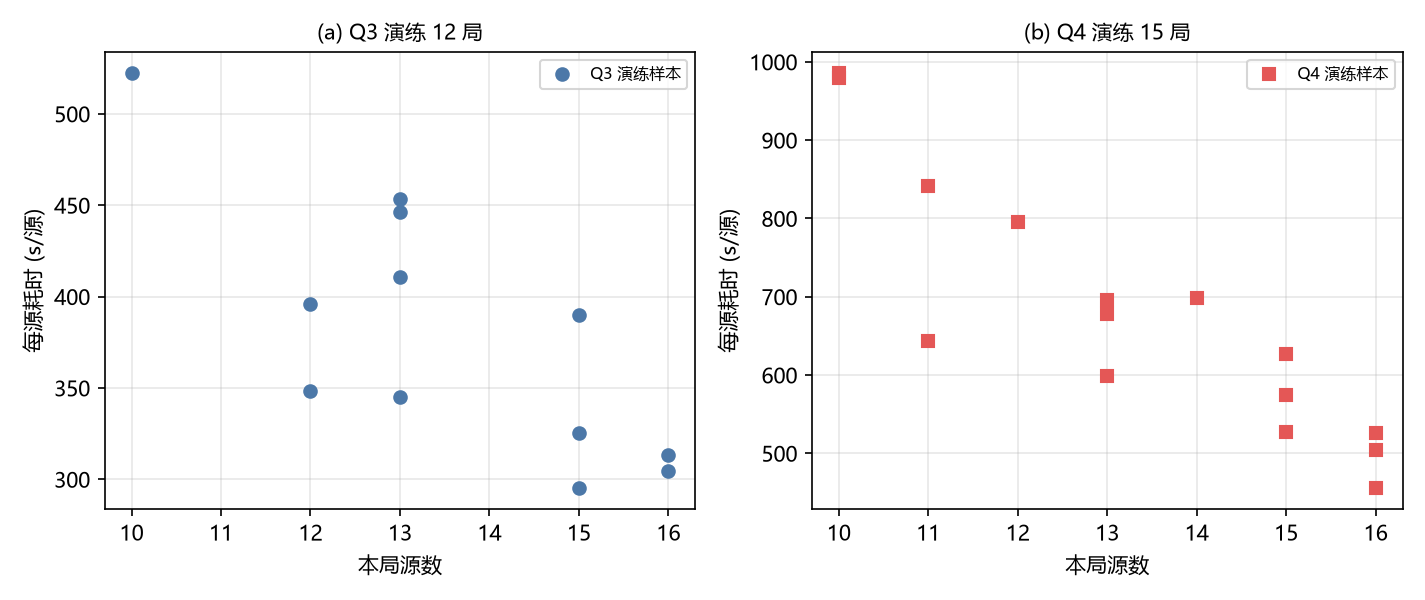
\includegraphics[width=\textwidth]{fig11.png}
  \caption{27 局真机演练的逐局散点（数据自演练登记表）：每源耗时随本局源数增加被摊销下移，相近源数的局间波动约 $\pm 10\%$。}
  \label{fig:scatter}
\end{figure}

\subsection{阈值敏感性（配对种子、单变量）}

所有敏感性实验均为配对种子离线实验：同一批随机种子下只改动单变量，差值可归因于该变量本身（图 \ref{fig:sens}）。

\begin{itemize}[leftmargin=2em,itemsep=3pt]
  \item \textbf{Q3 收敛即清距离闸}：闸值取 $0,150,400,600,800\,$m 时每源耗时依次为 398.4、360.8、359.4、359.8、$363.9\,$s，其中 $150\sim 600\,$m 为平台区，取值 $400\,$m 距最优 $0.4\,$s/源；禁用（0）代价 $+10.9\%$。
  \item \textbf{Q4 顺路清除绕路上限}：上限取 $200,300,400,600,800\,$m 时依次为 738.7、735.7、734.4、737.6、$745.4\,$s，曲线呈光滑 U 形，谷底恰在取值 $400\,$m 处。
  \item \textbf{Q4 补测几何参数}：深度、横移距离、侧序等 8 组变体的扰动影响在 $\pm 0.1\%$ 量级，补测几何远离敏感区。
  \item \textbf{Q4 布局}：见 5.4.5 节布局对照（$-18.3\%$，真机 $-14\%\sim-23\%$）。
\end{itemize}

\begin{figure}[H]
  \centering
  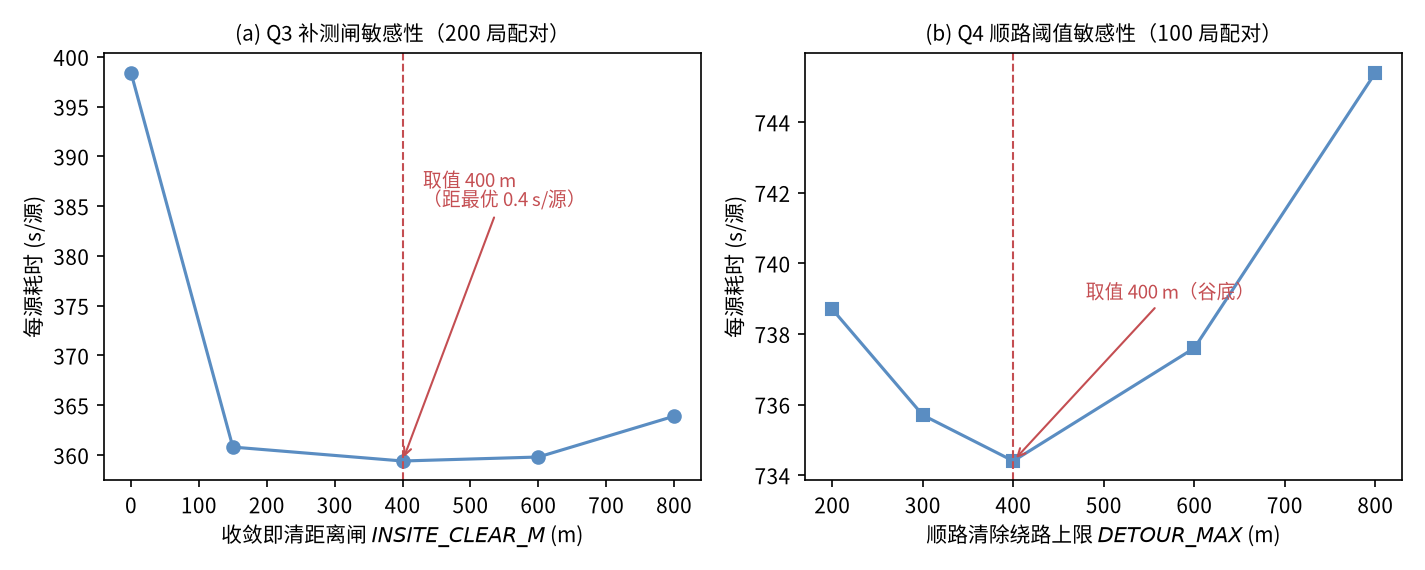
\includegraphics[width=\textwidth]{fig12.png}
  \caption{两个关键阈值的配对种子敏感性扫描：均处于平台区/谷底，参数选择对扰动不敏感。}
  \label{fig:sens}
\end{figure}

\subsection{异常与故障回归}

故障注入回归对 \verb|measure|/\verb|clear|/\verb|exit| 三类接口注入动作被拒与网络重试耗尽两类故障（覆盖搜索、补测、兜底各阶段，共 100 项），断言分类完备性等不变式，全部通过；时间不足（\verb|remaining = 1 s|）注入下程序正常降级退出、summary 完整。需要说明的验证边界：离线回归只累计虚拟时间，时间保护分支仅验证了正确进入，未在真实网络竞争下验证保护效果；单请求最坏真实耗时约 $25\,$s（$8\,$s 超时 $\times$ 3 次重试加退避），各阶段 $150\sim 300\,$s 的时间预留可容忍连续多次最坏请求。

\subsection{正式测试结果}

\begin{table}[H]
  \centering
  \caption{正式测试逐局结果（2026-09-12；脚本 md5 与提交版本一致，脱敏逐局日志见支撑材料）}
  \label{tab:formal}
  \begin{tabular}{lccccccc}
    \toprule
    局 & 源数 & 清除 & 虚拟时间 & 每源耗时 & 测量/清除次数 & 真实耗时 \\
    \midrule
    Q3-1 & 12 & 12/12 & $4667.5\,$s & $389.0\,$s/源 & 151/12 & $1.2\,$s \\
    Q3-2 & 12 & 12/12 & $4679.2\,$s & $389.9\,$s/源 & 162/12 & $1.2\,$s \\
    Q3-3 & 16 & 16/16 & $5339.1\,$s & $333.7\,$s/源 & 153/16 & $1.2\,$s \\
    \midrule
    \textbf{Q3 小计} & \textbf{40} & \textbf{40/40} & --- & \textbf{367.1\,s/源} & --- & --- \\
    \midrule
    Q4-1 & 10 & 10/10 & $6978.0\,$s & $697.8\,$s/源 & 314/10 & $2.2\,$s \\
    Q4-2 & 13 & 13/13 & $6294.7\,$s & $484.2\,$s/源 & 291/13 & $1.8\,$s \\
    Q4-3 & 14 & 14/14 & $7085.3\,$s & $506.1\,$s/源 & 273/14 & $1.6\,$s \\
    \midrule
    \textbf{Q4 小计} & \textbf{37} & \textbf{37/37} & --- & \textbf{550.2\,s/源} & --- & --- \\
    \bottomrule
  \end{tabular}
\end{table}

六局全部被模拟器接受退出（exit accepted）、\textbf{零拒绝动作}、\textbf{零失败信道}；兜底层全程零触发。正式成绩与离线回归、演练水平的吻合度见表内数字与 6.1 节。

%========================== 七、模型的评价与推广 ==========================
\section{模型的评价与推广}

\subsection{主要优点}

\begin{enumerate}[leftmargin=2em,itemsep=3pt]
  \item \textbf{保证与验证分层}：哪些结论是确定性命题（Thales 判据、弧判据、$19.75\,$m 闸、细网格夹逼不等式）、哪些由实验验证（定位清除成功率），全文口径统一，不混用。
  \item \textbf{参数选择全部有实验依据}：MEC 圆心补测（$-10.6\%$ 消融）、收敛即清闸（平台区）、顺路上限（U 形谷底）、布局（400 局配对 $+$ 真机同源数配对）均为配对实验：实验中保持随机案例与其他模型组件一致，仅改动单一变量，减少场景差异对比较结果的干扰。
  \item \textbf{工程鲁棒性}：异常降级语义使任何单点故障不弃局，故障注入 100 项验证；真机 33 局 440/440 的实测记录支撑结论。
  \item \textbf{连续域证据链完整}：弧判据先经三条独立数值通道交叉复核，再按主体区、检出圆条带、测站邻域和边界交点邻域分层闭合；程序输出记录每层点数、最小闭包量和最终 \verb|all_closed=true|。
\end{enumerate}

\subsection{主要缺点}

\begin{enumerate}[leftmargin=2em,itemsep=3pt]
  \item \textbf{问题三无清除兜底层}：单信道 8 次补测用尽即计入 \verb|failed_channels|，理论上存在近平行薄楔病态构型使定位收敛失败且无对应对物；800 局离线与真机均未触发，风险极低但机制上未封堵（问题四已用细网格封堵同类缺口）。
  \item \textbf{问题四证明采用分层数值认证}：连续域结论依赖分层网格、Lipschitz 界与近站邻接弧解析界，而非一个简短的全解析闭式证明；复现成本较高，必须随附逐层日志和机器可读结果。
  \item \textbf{问题二目标为样本意义}：$\Phi$ 的凸性未证明，最坏值靠边界与内部联合采样估计，报告的是加密离散样本下的最优，非连续域严格最优；严格化需区间分支定界。
  \item \textbf{时间保护未在真实竞争下检验}：真实耗时保护分支未经历过网络持续劣化的实测，仅验证了逻辑正确与预算裕度。
\end{enumerate}

\subsection{改进方向}

针对缺点 1，可把问题四的细网格兜底按信道可行域裁剪后移植到问题三（问题三全向源无需前向半平面约束，网格可更稀）；针对缺点 2，弧判据可对 26 点骨架的对称类做完整分情形解析证明，或采用经区间算术认证的分支定界；针对缺点 3，用区间分析对 $\Phi$ 做分支定界可得连续域严格上界。

%========================== AI 工具使用说明 ==========================
\section*{AI 工具使用说明}
\addcontentsline{toc}{section}{AI 工具使用说明}

本队按照《全国大学生数学建模竞赛人工智能工具使用规定（2026 年试行）》声明：竞赛期间，我们使用生成式人工智能工具辅助完成了以下工作：(1) 离线模拟器与验证脚本（回归测试、故障注入、布局覆盖检查）的代码编写与调试；(2) 数值实验的组织与结果整理；(3) 论文初稿的文字整理与排版。全部模型的建模思路、口径选择、判据推导、参数取舍与结论检验由参赛队完成并逐项复核；所有数值结果均可由支撑材料中的源程序与日志复现，AI 未生成任何未经我们验证的数据或结论。

%========================== 八、参考文献 ==========================
\section{参考文献}

\begin{enumerate}[leftmargin=2.2em,itemsep=3pt,label={[\arabic*]}]
  \item BISHOP A N, FIDAN B, ANDERSON B D O, et al. Optimality analysis of sensor-target localization geometries[J]. Automatica, 2010, 46(3): 479-492.
  \item NARDONE S C, LINDGREN A G, GONG K F. Optimal observer motion for localization with bearing measurements[J]. Computers \& Mathematics with Applications, 1989, 18(1-3): 171-180.
  \item ZHAO S, CHEN B M, LEE T H. Optimal placement of bearing-only sensors for target localization[C]//Proceedings of the American Control Conference. IEEE, 2012: 27-32.
  \item JAULIN L. Set-membership localization with probabilistic errors[J]. Robotics and Autonomous Systems, 2011, 59(6): 489-495.
  \item LIU Y S, ZHAO Y, WU F L, et al. Bearing-only target tracking based on ellipsoidal outer-bounding set-membership estimation[J]. Journal of Beijing University of Aeronautics and Astronautics, 2017, 43(3): 497-505.
  \item CHOSET H. Coverage for robotics---a survey of recent results[J]. Annals of Mathematics and Artificial Intelligence, 2001, 31(1-4): 113-126.
  \item GALCERAN E, CARRERAS M. A survey on coverage path planning for robotics[J]. Robotics and Autonomous Systems, 2013, 61(12): 1258-1276.
  \item GABRIELY Y, RIMON E. Competitive on-line coverage of grid environments by a mobile robot[J]. Computational Geometry, 2003, 24(3): 197-224.
  \item CROES G A. A method for solving traveling-salesman problems[J]. Operations Research, 1958, 6(6): 791-812.
  \item POPOVI\'{C} M, OTT J, R\"{U}CKIN J, et al. Learning-based methods for adaptive informative path planning[J]. Robotics and Autonomous Systems, 2024, 174: 104627.
  \item LEE T K, BAEK S H, CHOI Y H, et al. Smooth coverage path planning and control of mobile robots based on high-resolution grid map representation[J]. Robotics and Autonomous Systems, 2011, 59(11): 801-812.
\end{enumerate}

%========================== 附录 ==========================
\appendix
\ctexset{
  section = {name={附录\hspace{0.2em},}, number=\Alph{section},
             format=\centering\bfseries\zihao{4}, aftername=\hspace{0.6em}},
  subsection = {number=\Alph{section}.\arabic{subsection}},
}

\section{支撑材料文件清单}

支撑材料压缩包包含以下文件（与论文内容一致）：

\begin{itemize}[leftmargin=2em,itemsep=2pt]
  \item \verb|robot_q3_v2.py|：问题三在线程序（正式测试版本，md5 b6631804）；
  \item \verb|robot_q4.py|：问题四在线程序（正式测试版本，md5 c1c77732）；
  \item \verb|q1_core.py|、\verb|q1_run.py|：问题一判据与数值实验；
  \item \verb|q2_model.py|：问题二鲁棒选点模型；
  \item \verb|offline_test_v2.py|、\verb|q4_offline.py|：问题三/四离线回归；
  \item \verb|fault_injection_test.py|：故障注入回归（100 项）；
  \item \verb|q4_layout_26_check.py|、\verb|q4_boundary_sliver_check.py|、\verb|q4_layout_tri_check.py|：布局验证与边界薄缝检查；
  \item \verb|q4_strip_check.py|、\verb|q4_closure_pointwise.py|：无盲区结论的四层采样与 Lipschitz 闭合检查（结果文件 \verb|all_closed=true|）；
  \item \verb|q4_fallback_trigger_test.py|：兜底强制触发单测；
  \item 逐局日志 \verb|logs-anon/|（\verb|robot-q3-formal-*-anon.jsonl|、\verb|robot-q4-formal-*-anon.jsonl|，已去除 \verb|robot_id| 字段以满足匿名评审要求）。
\end{itemize}

\section{主要源程序}

以下为两问正式测试版本的完整源代码，与提交的支撑材料一致；按竞赛要求，附录中仅保留代码本身，所有注释与文档字符串已去除（支撑材料中的原件含完整注释，可对照阅读）。

\subsection{问题三程序 \texttt{robot\_q3\_v2.py}}

\lstinputlisting[language=Python]{code/robot_q3_v2.py}

\subsection{问题四程序 \texttt{robot\_q4.py}}

\lstinputlisting[language=Python]{code/robot_q4.py}

\end{document}
